\chapter{时空注意力机制的视频显著性检测方法}
\renewcommand{\leftmark}{第三章\quad 时空注意力机制的视频显著性检测方法}

\section{引言}
在上一章节中,本文提出了基于弱监督学习的深度级联网络(SCNN)来完成视频显著性目标检测。SCNN通过结合深度网络生成的静态先验和基于光流生成的动态先验来引导网络学习。面对训练数据不足,SCNN则提出了并行迭代弱监督的训练策略,使得SCNN网络可以顺利地学习鲁棒的显著特征。虽然SCNN的方法取得了很好的成果,但是也存在一些特殊情况SCNN解决不了,并且这些特殊情况也限制了显著性检测的进一步提高。

本文研究视频显著性检测的一大的动机就是运动特征不好通过传统的深度模型进行学习,因此在SCNN中使用了外部运动特征引入的方法,利用光流图超像素分割提取运动区域,再利用深度特征生成运动先验图,并融合静态先验后引导级联深度网络学习。这一个融合的时空先验被证明是有效的,但是仍存在问题,即无论的静态先验还是运动先验都需要保证图像的主体显著区域需要被检测出来。只要有一个先验图没有检测到显著目标,则其先验图显著区域即为空值,再使用像素级相乘,那么融合后的时空先验也会是空值,这样的空值先验是不会对网络学习又促进作用,反而会抑制网络学习显著性特征。也可能存在一些极端的情况,就是两个先验图是互补的情况,即各自检测出显著目标的一半,二者相乘则整个先验图都为空值,从而导致级联网络学习不到任何东西,使得显著检测失败。

第二大动机就是训练数据不足。SCNN则是引入弱监督的学习方法生成大量的弱标签来完成网络训练。然而,生成的弱标签仍存在不小的问题。由于生成的弱标签主要采用融合静态显著图的方法,这些静态的图像显著性检测方法主要是处理图像显著性的,不具有任何运动特性,再加上显著性视频数据场景变化多样,所以融合而成的弱标签图时存在一些背景噪声。即使在SCNN网络训练时,本文提出的并行迭代弱监督的训练策略,在复杂场景下的背景噪声仍然存在。因此,像素级标签的质量需要进一步提升。

在本章内容中,针对这二个难点,本文分别提出了有效的方法来解决这两个问题。首先是训练数据不足问题。既然弱标签不准确且存在背景噪声,解决问题的最好方法还是直接标定。通过尝试我们发展标记一张像素级实在太消耗时间,但是如果在从弱标签中擦除背景噪声比较容易,也节省时间。因此,本文没有直接从视频帧上标定像素级标签,而是从融合的显著图上擦除背景噪声,这样擦除背景噪声后的标签图本文称为粗标签。粗标签虽然没有真实的像素级标签精细,但是其保留了正确的显著性区域,而且没有背景噪声,只是在显著目标周围边界略显粗糙。本文标记了一定数量的粗标签,并且利用这些标签训练取得了很好的效果。

其次,针对运动特征不好学习的问题,本文提出了时空双流网络和引入多种运动特征精炼模块,分别从运动先验和视频序列中提取运动特征。时空双流网络主要针对SCNN中时空先验的不足,由于时空先验是使用像素级矩阵相乘的方法融合静态与运动先验,但是在特殊情况下得到的先验会是空值,不能引导网络做进一步的学习。为了避免这类情况,本文在SCNN级联网络的基础上,提出了一种新型的并行双流网络,一个子网流采用静态视频帧作为输入,主要用以提取静态特征。另一个子网流则采用运动先验与视频帧的组合作为输入,主要用以提取运动特征。之后,再在网络的后端进行特征融合进而完成显著性估计。于此同时,为了进一步挖掘视频序列中的运动特征,本文引入了两种运动特征精炼模块,分别为LSTM和3D卷积,通过输入连续特征图序列的方式进一步挖掘运动特征。

最后,由于此方法采用新型的双流网络结构和引入了两个运动精炼模块,因此产生多类型的特征图。如何融合这些多类型的特征图也是需要探索的问题。良好的特征融合方法可以很好地探索多类型特征之间的相关性和互补性,从而生成鲁棒性高的融合特征。在刚开始时,本文仍是采用简单直接的方法,采用分级特征图相加的方式融合,即先融合双流子网生成的多尺度特征图,再融入运动精炼模块的特征图。之后,为了进一步探索多类型特征之间的相关性和互补性,本章又引入一个注意力机制来融合这些特征。注意力机制的原理是采用学习的方式,计算输入特征图的相关性,从而生成针对每一个类型特征图的权重,最后再利用加权求和完成特征的融合。

总结来说,本章提出的方法总共有以下贡献:
\begin{itemize}
  \item 本文提出了一个新颖的双流子网模型(STAN),该模型巧妙地避免的融合时空先验的弊端,采用空间、时间双子网的方式分别提取不静态与运动特征。
  \item 为了克服网络训练不足,本文又标定一定数量的粗像素级标签,该标签虽然需要人工操作,但是效率很高,而且比SCNN中的并且弱监督方法生成弱标签准确,从而避免在复杂场景下弱标签背景噪声的干扰。
  \item 在视频显著性检测中,运动特征的提取至关重要,本文在运动先验之后,又引入多种运动特征精炼模块(LSTM和3D卷积)生成不同类型的神经网络特征图,并在STAN的网络末端加入一个基于注意力机制的特征融合模型,使得模型可以学习到特征之间的相关性和互补性,进而得到鲁棒的融合特征。
  \item 本文在广泛使用的数据集FBMS和DAVIS的实验表明,STAN比之前SCNN的效果更好,也能处理更为复杂的视频运动场景。
\end{itemize}

在本章中,我们把内容分为引言,主要分析研究本章内容的动机、面临的困难和提出解决困难的方法。然后的详细方法描述,其中包括绍多尺度特征的卷积LSTM网络、基于注意力特征融合的深度网络、注意力融合模块和粗标签的生成。接着是实现的验证和详细的分析。最后是对本章内容的总结。

\section{方法描述}
\subsection{多尺度特征的卷积LSTM网络}
本章的深度网络存在两个阶段的发展,首先是多尺度特征的卷积LSTM网络(MSST),其网络结构三个部分:空间子网、时间子网和卷积性LSTM(ConvLSTM)模块。空间子网是由改进型的全卷积VGGNet组成,与SCNN一样在最后的两个卷积块中引入了膨胀卷积来保持卷积运算时的感受野。时间子网与空间子网的结构几乎一样,唯一的不同即为网络输入。在空间子网中,网络输入是连续的RGB视频帧,而时间子网的网络输入则为RGB视频帧与其对应运动先验的组合。在网络前向的过程中,本文还在网络中设计了多个分支,分别提取两个子网的多尺度特征图。之后,再把这些时序的多尺度特征图输入到ConvLSTM模块,用以精炼运动特征。最后,空间子网、时间子网和ConvLSTM模块生成的特征图,利用一个卷积核为1$\times$1的卷积直接在网络的后端进行融合,生成最终的显著检测图。

\begin{figure*}
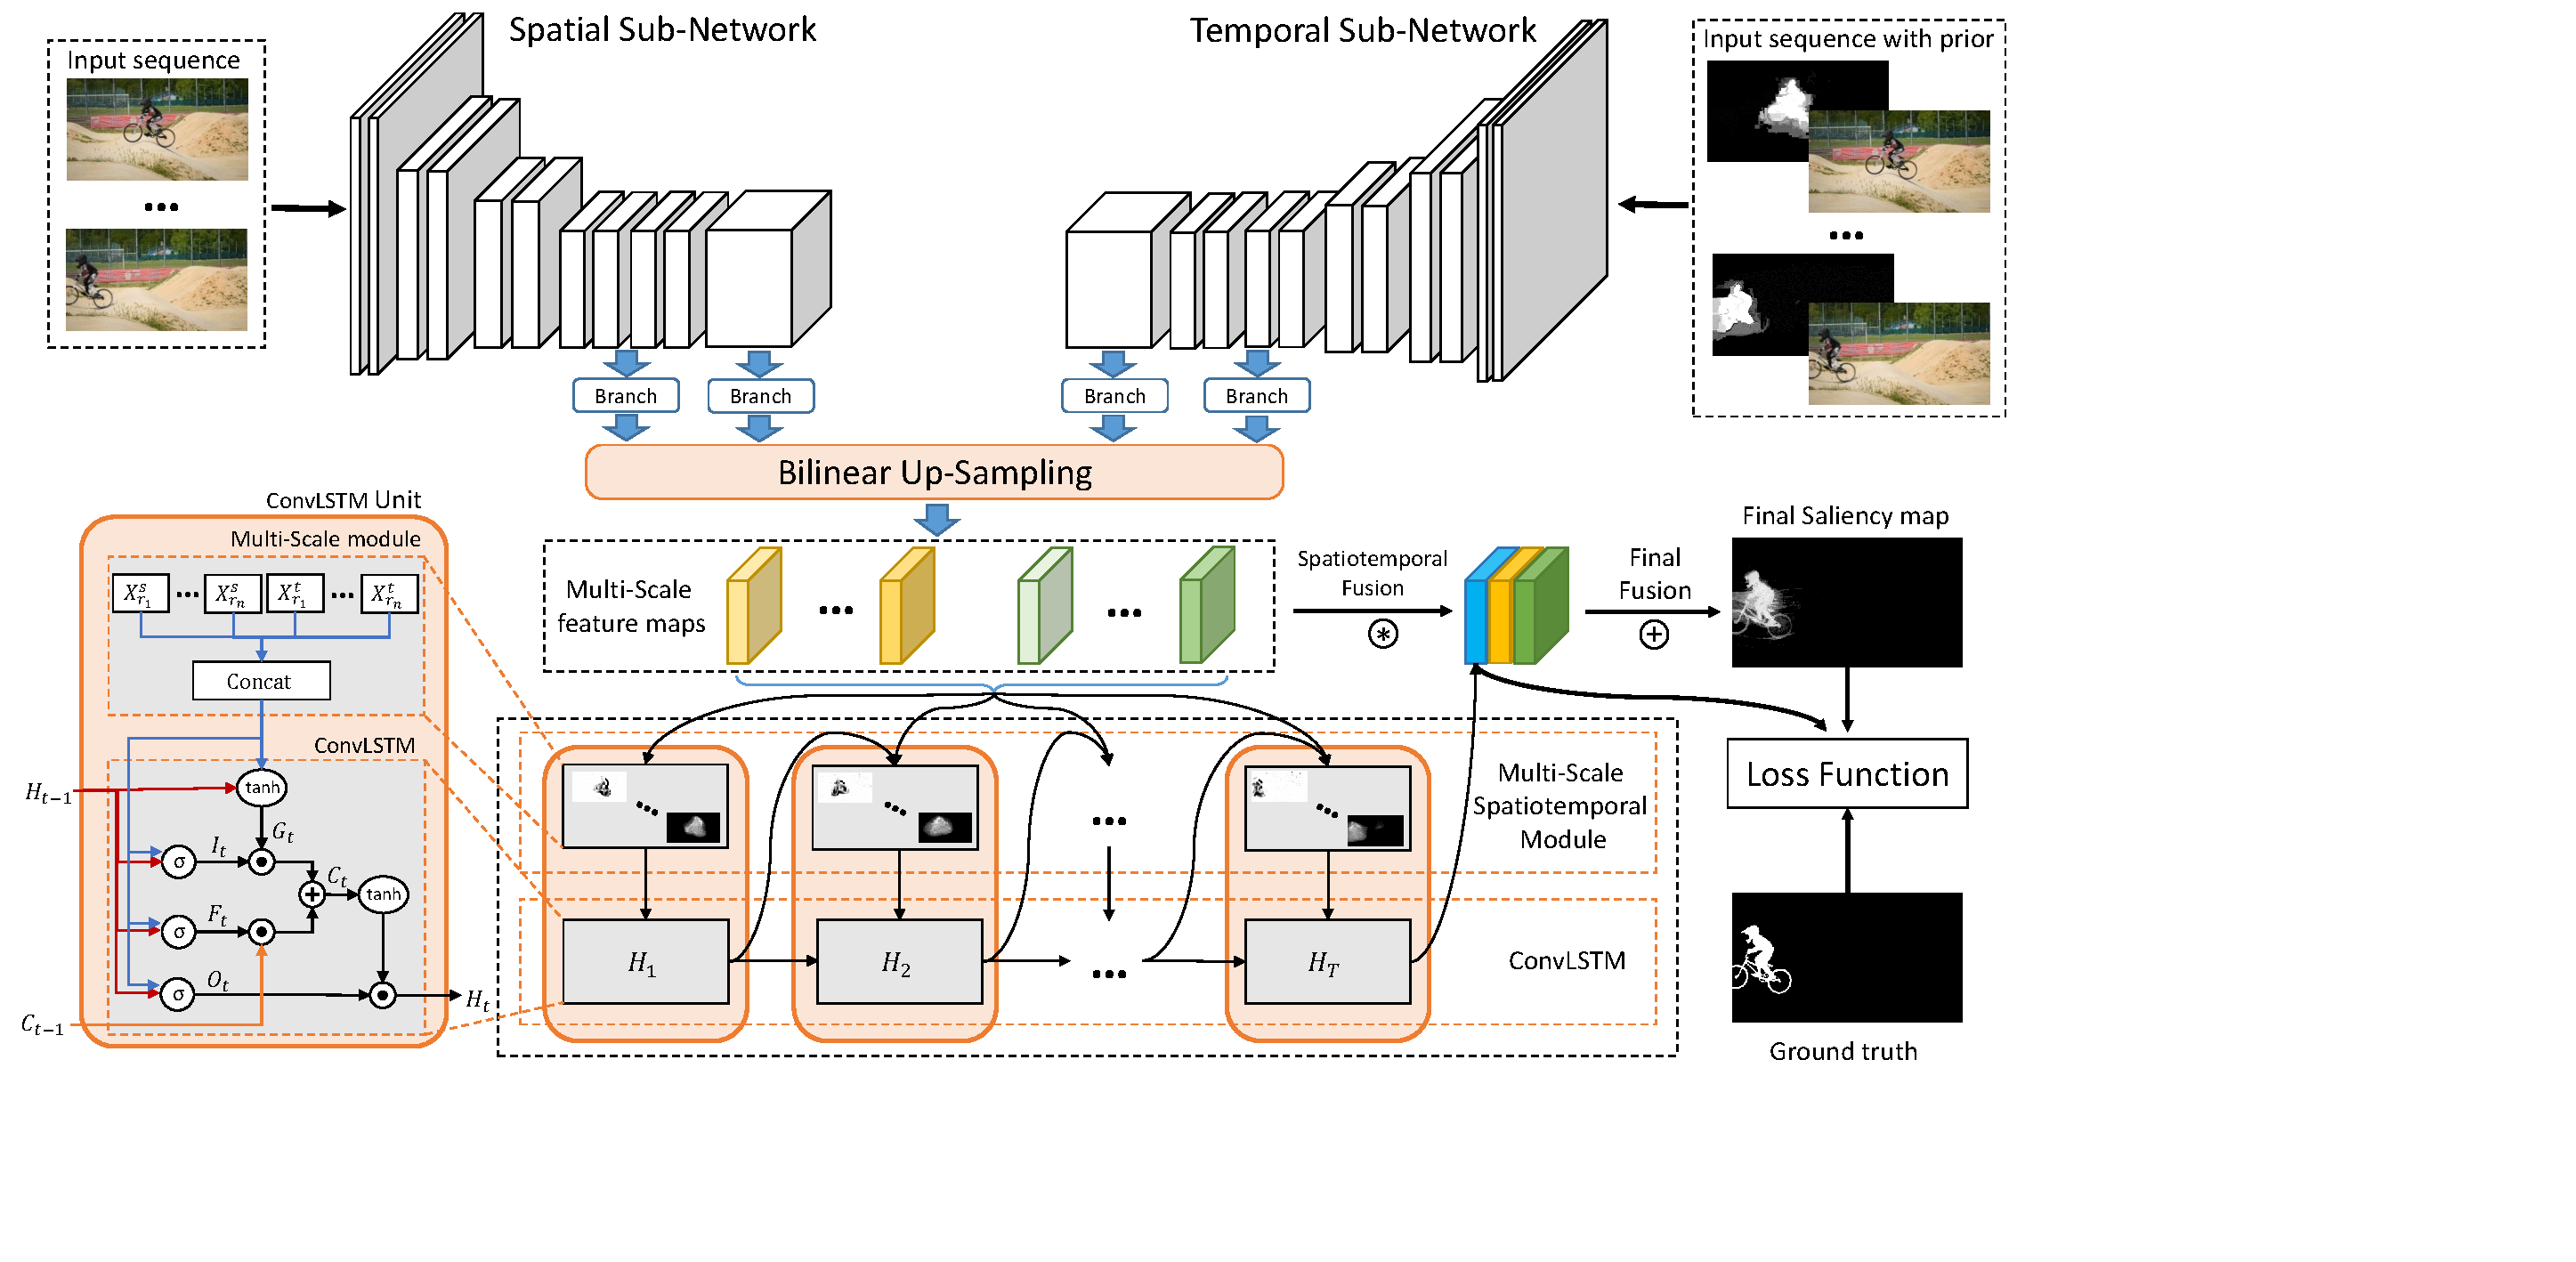
\includegraphics[width=15cm]{figures/msst_framework}
\caption{级联深度的结构图}
\label{msst}
\end{figure*}

多尺度特征的卷积LSTM网络的具体结构如图\ref{msst}所示。同样的,与SCNN一样的基于VGGNet的全卷积结构,包括五个pooling层,使得卷积操作的感受野逐渐增大。并且,这五个pooling层也把VGGNet的所以卷积分成六个卷积块。为了保证合适卷积感受野,本文修改的pooling的参数,把步长从原来的2变成了1。此外膨胀卷积也嵌入到VGGNet中后两个卷积块。同时,为了得到多尺度的特征图,本文设计了两个卷积分支,该分支由一个128通道、卷积核为3$\times$3的卷积层和一个1通道、卷积核为1$\times$1的卷积层构成,并被嵌入到第四个卷积块和最后一个卷积块后。这些多尺度特征图在利用上采样层,调整大小与输入图像一致后,再输入进ConvLSTM模块进行运动特征精炼。

在图\ref{msst}的左下角有本文引入的卷积性LSTM的具体框架图。这一结构具体由多尺度时空特征融合模块和卷积LSTM模块组成。先给定两个子网的网络输入$I^s$和$I^t$,双子网的多尺度特征提取可以总结为:

\begin{equation}
 \label{eq3_4}
 \begin{aligned}
 \quad X^{s}_{r_i} &=  U^{s}_{r_i}(F^{s}_{r_i}(I^s;\theta^{s}_{r_i})) \\
        \quad X^{t}_{r_i} &=  U^{t}_{r_i}(F^{t}_{r_i}(I^t;\theta^{t}_{r_i})), i \in \{1, 2, ..., n\}
 \end{aligned}
\end{equation}

其中,$X^{s}_{r_i}$和$X^{t}_{r_i}$分别表示在不同尺度$r_i$下,空间子网和时间子网生成所生成的特征图;$F^{s}_{r_i}(\cdot)$与$F^{t}_{r_i}(\cdot)$则是两个子网的卷积运算;$U^ {s}_{r_i}(\cdot)$与$U^{t}_{r_i}(\cdot)$则为两个子网的线性上采样操作。在完成多尺度特征提取之后,所有的特征图用Concatenation操作(Con)堆叠成$X^\tau $ ($\tau  \in \{1, 2, ..., T\}$):

\begin{equation}
 \label{eq3_3}
 \begin{aligned}
    X^\tau  = \textbf{Con}(X^{s}_{r_1}, ...,X^{s}_{r_n},X^{t}_{r_1}, ...,X^{t}_{r_n})\\
 \end{aligned}
\end{equation}

$X^1, ..., X^T$这些堆叠的特征图(T为时间间隔,即一个网络输入包含T个视频帧内)会被送入ConvLSTM模块用以精炼运动特征。ConvLSTM的运算可以看成是一组卷积运算,归纳为

\begin{equation}
\label{P_motion}
\begin{aligned}
   O_{m}  &= M(X^1, ..., X^T; \theta_m)
 \end{aligned}
\end{equation}

其中$M$为ConvLSTM运算集合;$O_{m}$为其输入的特征图;$\theta_m$是ConvLSTM对应的学习参数。事实上,ConvLSTM可以展开为了一个门运算,包括:输入门$I_t$、遗忘门$F_t$和输出门$O_t$,其完整的计算方式可以表示为:

\begin{equation}
\label{s_lstm}
\begin{aligned}
   I_{t}  &= \sigma(W_{xt} * X_t + W_{ht} * H_{t-1} + b_i) \\
   F_{t}  &= \sigma(W_{xf} * X_t + W_{hf} * H_{t-1} + b_f) \\
   O_{t}  &= \sigma(W_{xo} * X_t + W_{ho} * H_{t-1} + b_o) \\
   C_{t}  &= F_{t} \circ C_{t-1} + I_{t} \circ tanh(W_{xc}* X_t + W_{hc} * H_{t-1} + b_c) \\
   H_t &= O_t \circ tanh(C_t)
 \end{aligned}
\end{equation}

公式\ref{s_lstm}中,$W_{xt}$、$W_{xf}$、$W_{xo}$、$(W_{xc}$分别对应输入门、遗忘门、输出门、状态节点与当前第t帧输入特征图$X_t$运算的卷积参数,而$W_{ht}$、$W_{hf}$、$W_{ho}$、$W_{hc}$则分别对应与前一帧隐变量$H_{t-1}$的卷积参数;$b_i$、$ b_f$、$ b_o$、$ b_c$分别是各个卷积运算的偏置项;`$*$'表示的是卷积运算,而`$\circ$'表示的哈达玛积,即对应元素相乘。

从公式中,我们可以推断ConvLSTM运算可以“记忆”前一帧的状态,并通过遗忘门有条件地往下一帧传递有用的信息。在视频显著性领域,这一计算方式就尤为突出,可以很好地提炼隐藏在视频序列中的显著性信息。

在完成ConvLSTM运动特征精炼之后,加上之前双流子网络提取到的多尺度空间、时间特征。在网络的后端,MSST可以得到三种不同类似的特征图:空间子网特征图、时间子网特征图和ConvLSTM运动精炼特征图。由于三者的特征类型不同,所以涉及到多特征融合,本文在MSST网络中采用的一种渐进式直接融合的方法进行特征融合。具体的融合方式可以表示为:

\begin{equation}
\label{fuse_feat}
\begin{aligned}
   S  &= W^s * X^s + W^t * X^t + O^m \\
   X^s &= Con(X^s_{r_1}, ...,X^s_{r_i}, ..., X^s_{r_n}) \\
   X^t &= Con(X^t_{r_1}, ...,X^t_{r_i}, ..., X^t_{r_n}) \\
   i &\in \{1,2,...,n\}
 \end{aligned}
\end{equation}
在公式\ref{fuse_feat}中,S表示融合后直接生产的显著图;$X^s$和$X^t$分别表示为空间子网和时间子网堆叠在一起的多尺度特征图;$W^s$和$W^t$则是与空间、时间特征图对应的卷积参数;$O^m$则是通过ConvLSTM精炼后的运动特征图。通过这一公式,我们可以看到,渐进式求和就是先使用卷积(卷积核为1$\times$1)分别融合两个子网所产生特征图。接着,再使用元素相加的方法融合所有子网和ConvLSTM特征。这样的方法简单且实用,在保持不同类型特征各自特点的同时,试图学习到特征之间的相关性,在一定程度上完成的多类型特征的融合。然而,这样简单的相关性探索是不够的,随着特征类型的增多,这样简单直接的融合可能会造成特征的冗余,直接影响最终的显著性检测结果。因此,本文在之后为了探求更为合适的多类型特征的融合方法,引入的基于注意力机制的特征融合方法。
为了优化整个多尺度ConvLSTM网络,损失函数需要被引入,用来计算预测结果$S\in [0,1]^h*w*1$和真值$G\in [0,1]^h*w*1$($h$和$w$分别为输入视频帧的高与宽)之间的误差。同时,在MSST网络中,本文仍是使用二元交叉熵(sigmoid cross entropy)的目标函数来优化网络:

\begin{equation}
 \label{loss2}
 \begin{aligned}
   L_f(S, G) = &- \sum_{i=1} g_i \log P(s_i = 1|I^{s}_i, I^{t}_i; \Theta) \\
             &- \sum_{i=1} (1-g_i)\log P(s_i = 0|I^{s}_i, I^{t}_i; \Theta)
   \end{aligned}
\end{equation}

在公式\ref{loss2}中,$S$和$G$分别表示的是网络预测值和数据真值;$s_i$和$g_i$则分别表示网络预测值和数据真值中的一个像素点;$\Theta$表示整个网络待学习的参数;$P(\dot|\dot)$为预测的执行概率。

同时,为了加快ConvLSTM模块参数的训练,本文也还设计了一个辅助的二元交叉熵目标函数放在$L_r$,加上这一个辅助目标函数后,最终的优化函数可以表示为:

\begin{equation}
 \label{loss3}
 \begin{aligned}
   L = L_F(S,G) + \beta L_r(R,G)
   \end{aligned}
\end{equation}

其中,R是ConvLSTM模块的输出特征图;$\beta$是目标函数权重,这里本文设置为0.1。

\begin{figure*}
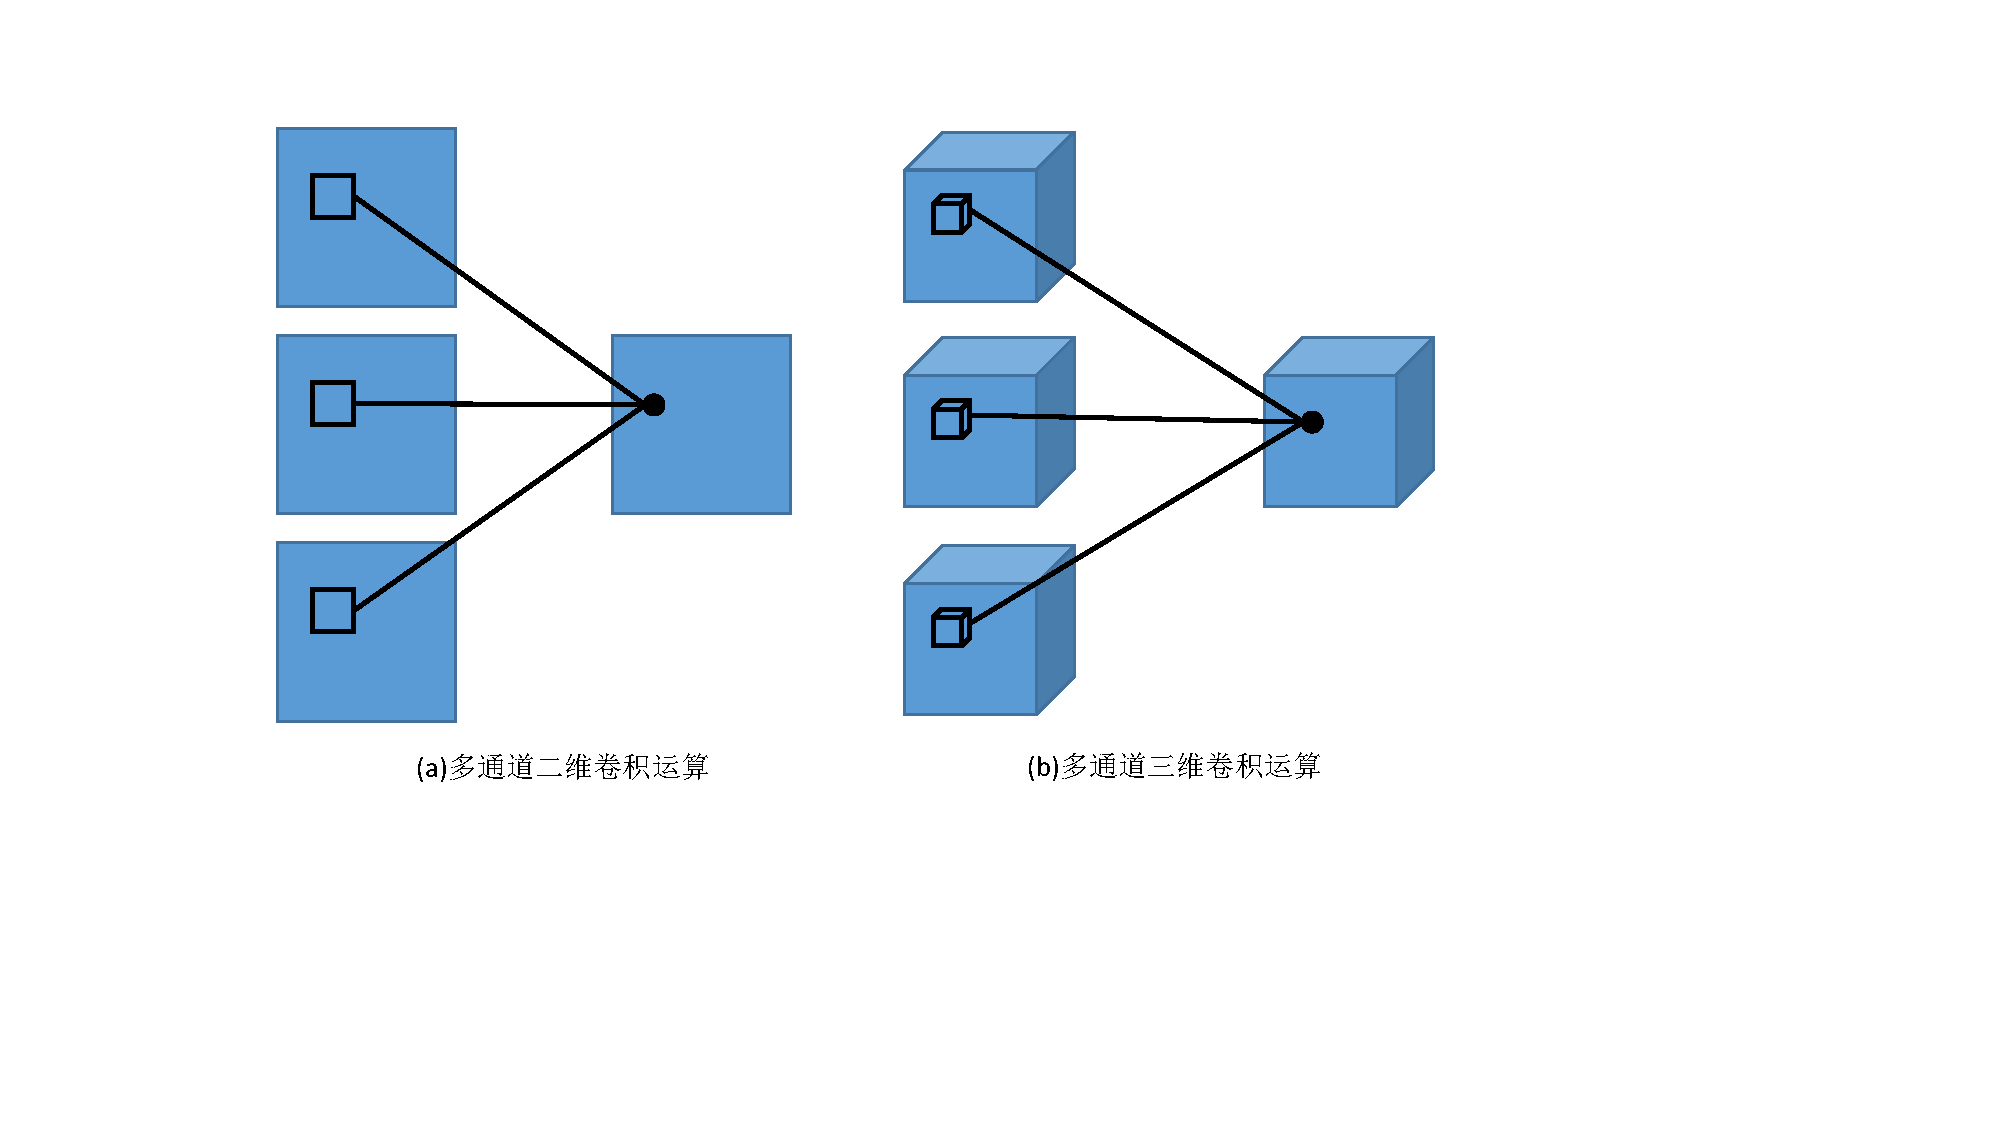
\includegraphics[width=15cm]{figures/2D3Dconv}
\caption{二维卷积与三维卷积比较}
\label{2d3dconv}
\end{figure*}

\subsection{基于注意力特征融合的深度网络}
基于注意力特征融合的深度网络是上述多尺度ConvLSTM网络(MSST)的改进。主要是在原有多尺度网络双流网络的基础之上,引入三维卷积操作,并与ConvLSTM组成一个运动特征精炼模块,并且在网络的末端,针对多类型的特征图的融合,提出了一种基于注意力机制的特征融合结构,从而生成比MSST网络更为优质的显著图。引入这两个模块的主要动机就是进一步挖掘隐藏在视频序列中的运动信息和探索多类型特征之间的相关性和一致性,进而生成更为鲁棒的深度特征。

相比针对图像处理的二维卷积,三维卷积的提出主要是针对处理连续的网络输入,进而挖掘序列的时序信息。三维卷积之所以有提取时序特征的能力是因此,相比于二维传统卷积,其输入特征图的大小和卷积核的大小都比二维卷积要多出一个维度。随着卷积核的滑动,三维卷积核即依次序列之间的特征图,得到的输出特征图是包含丰富的序列信息的。二维卷积核三维卷积的运算形式可以由图\ref{2d3dconv}说明:

图\ref{2d3dconv}(a)表现就是二维卷积运算,而图(b)则为三维卷积运算。我们看到,就输入而言二维卷积的输入是二维的,即输入尺度是(c,w,h),其中c是通道数,w与h分别是输入图像的宽和高。而三维卷积的输入则多了一个维度,其尺度是(c,w,h,d),其中d为图像深度。在进行卷积计算的时候,二维卷积的卷积核在滑动时,其计算范围是($k_w$,$k_h$),同理三维卷积在滑动时计算的范围是($k_w$,$k_h$,$k_d$)。通过引入一个额外的维度,三维卷积在计算时即可获得序列之间的信息。

\begin{figure*}
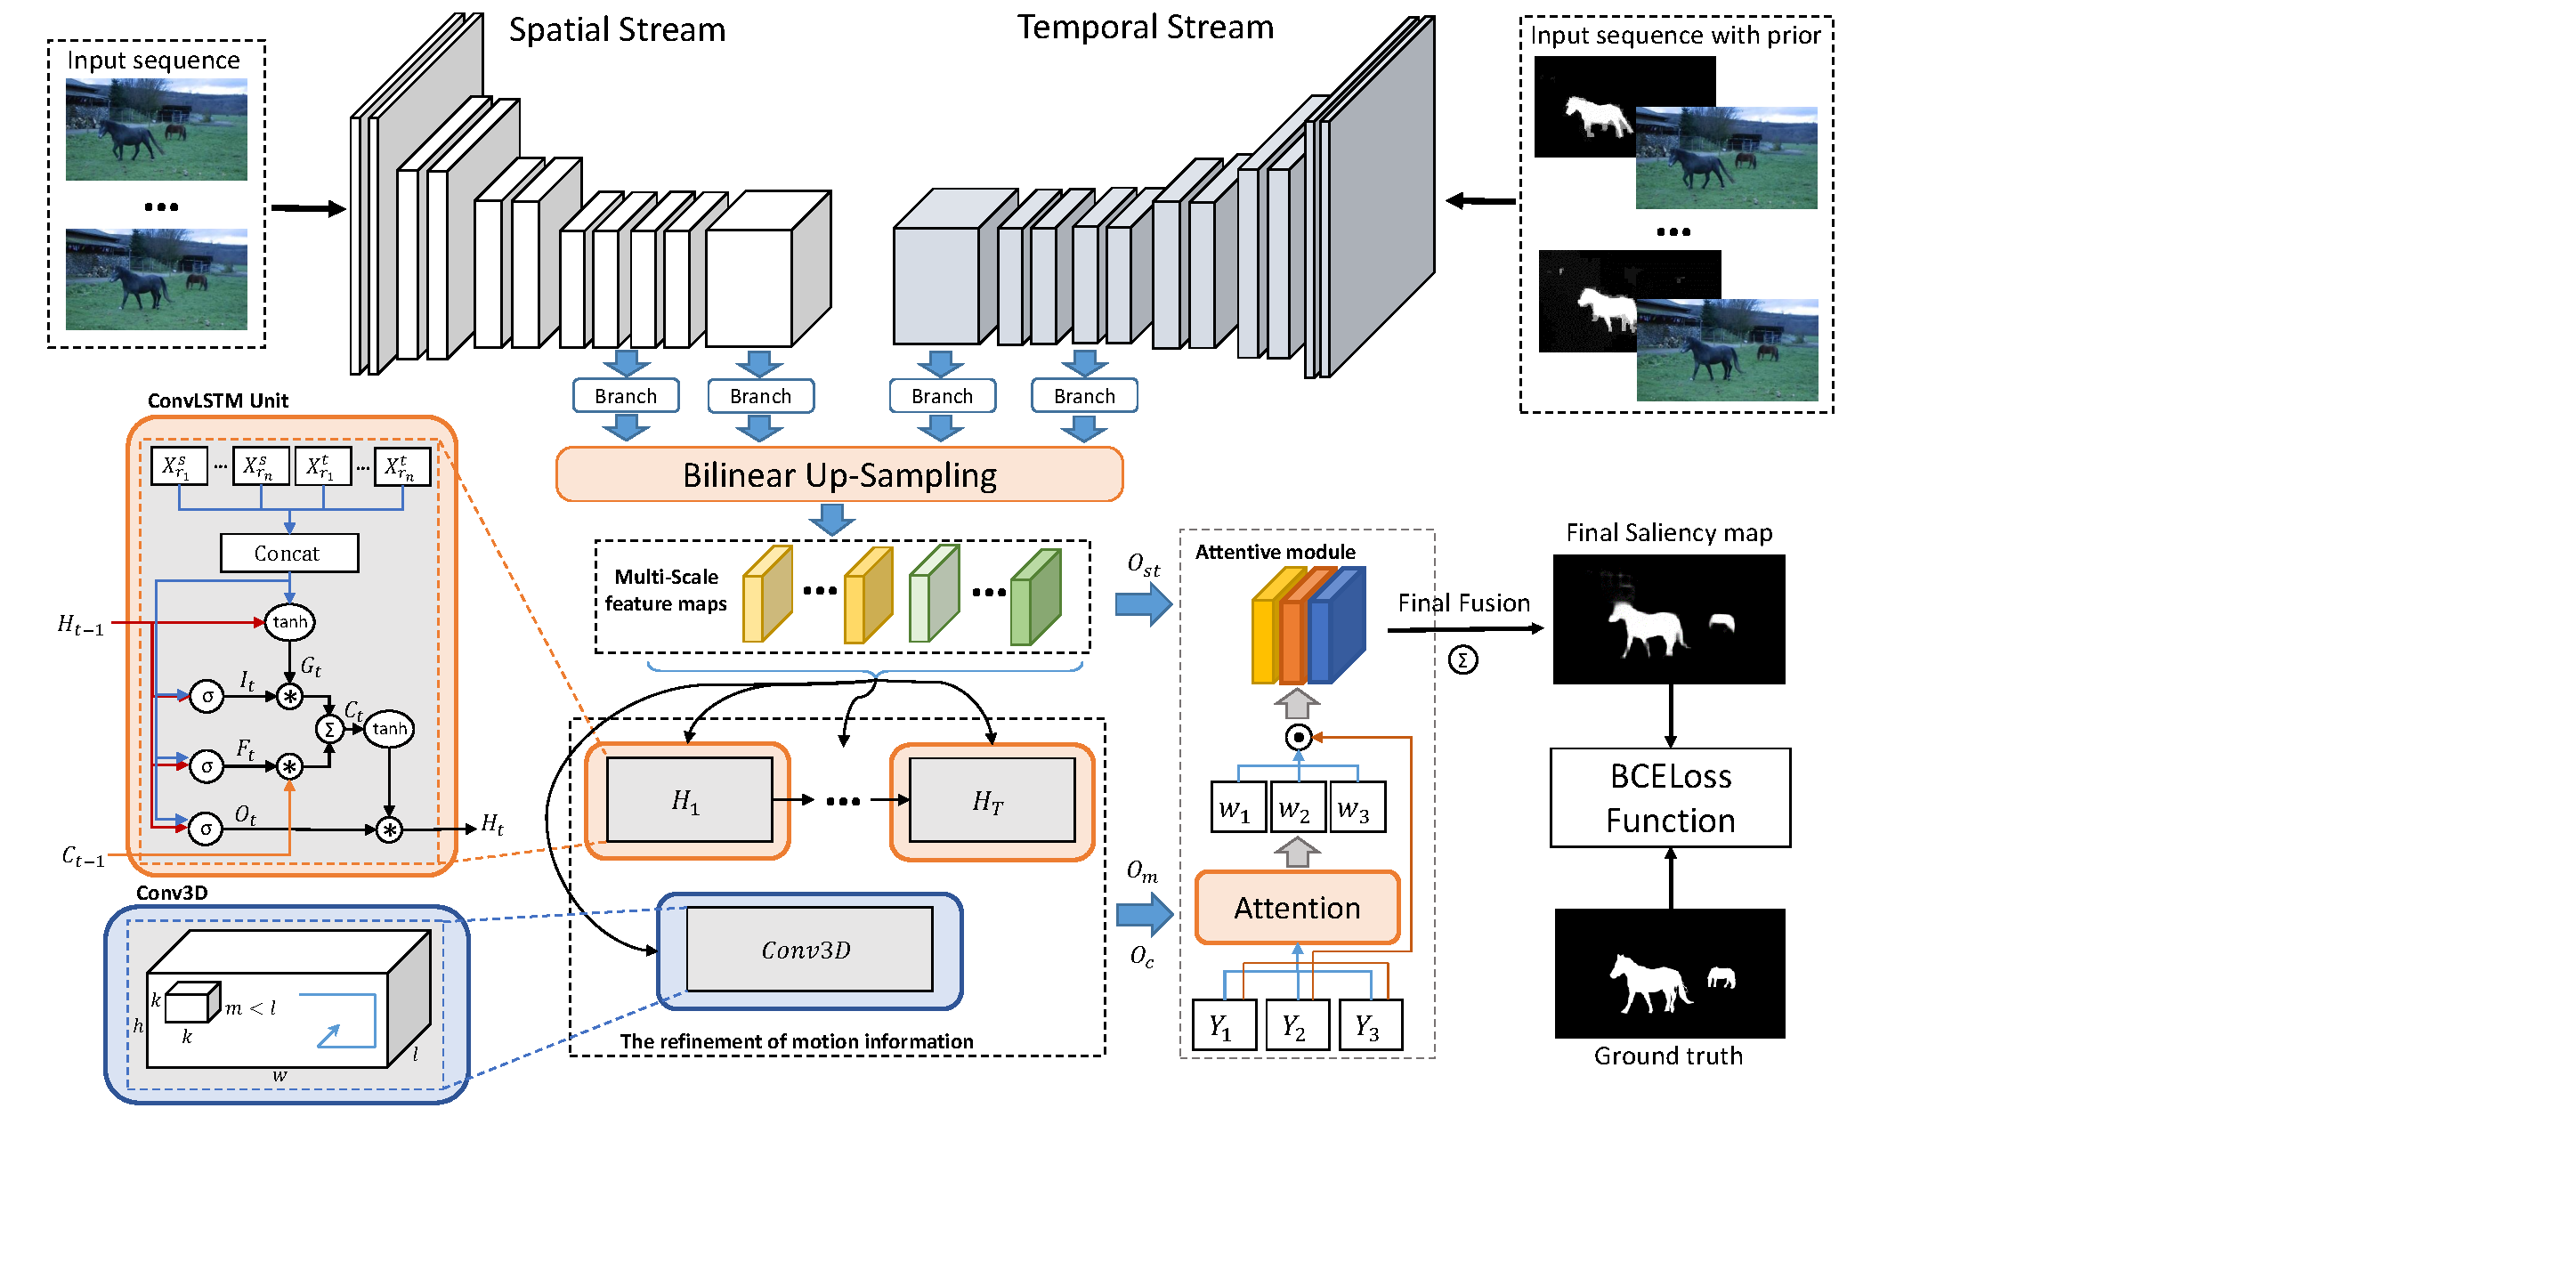
\includegraphics[width=15cm]{figures/stan_framework}
\caption{时空注意力机制的深度网络结构}
\label{stan}
\end{figure*}

在引入三维卷积和注意力机制后,时空注意力机制的深度网络如图\ref{stan}所示。原有的双流子网和多尺度特征提取是没有变化的,主要的变化在于原有的运动特征精炼只使用ConvLSTM,现在引入三维卷积操作与ConvLSTM分别精炼运动特征,即:

\begin{equation}
\label{P_motion}
\begin{aligned}
   O_{m}  &= M(X^1, ..., X^T; \theta_m) \\
   O_{c}  &= C(X^1, ..., X^T; \theta_c)
 \end{aligned}
\end{equation}

其中$O_{m}$与MSST的ConvLSTM是一样的,$O_{c}$则为三维卷积的输出,$C$为三维卷积操作;$\theta_c$是与之对应的卷积核参数。

与MSST模型一样,为了保持特征空间的一致性,双流子网流生成的多尺度时间与空间特征图需要先一步进行融合。采用的也是一个卷积核为1$\times$1的卷积层,然而再使用元素相加的哈达玛积,从而得到第一步的时空融合特征$O_st$:

\begin{equation}
\label{eq4_2}
\begin{aligned}
   O_{st}  &= \sum_{i}^{n} W^{st}_{r_i} * \textbf{Con}(X^{s}_{r_i} \ X^{t}_{r_i})
 \end{aligned}
\end{equation}

$X^{s}_{r_i}$与$X^{t}_{r_i}$即在不同尺度$r_i$上的特征图;$W^{st}_{r_i}$是对应需学习的卷积参数。第二步的特征融合就需要使用到本章提出的基于注意力机制的特征融合模块,把三个类型的特征图$O_st$、$O_m$、$O_c$融合成成鲁棒性更高的特征,进而生成比MSST网络更为准确的显著图(图\ref{stan}的右下角)。具体的注意力融合模块会下一个小节进行详细描述。在时空注意力机制网络的末端,仍是采用二元交叉熵目标函数(公式\ref{loss2})进行优化,并通过反向传播学习网络参数。

\subsection{注意力融合模块}
注意力机制是模拟人类注意力思维的方法,即人类通过快速地浏览图像、视频等事物,然后迅速在脑中浮现出那些最令人关注的区域(即权重最大处),之后再对这一个关注区域着重处理的过程。这一思路可以让人快速地定位到关键信息,并对这些信息进行重点处理,从而提高信息处理的效率和准确性。

注意力机制首先是应用到图像分类领域,在文献\cite{mnih2014recurrent}中,作者在循环神经网络(RNN)中率先使用注意力机制。在mnist手写数字图像中设计一个焦点作为注意力中心,通过循环迭代不断地更新焦点中心使其可以逐渐接近手写数字的中心,进而对数字中心的周围区域提取图像特征,完成图像分类。由于文献\cite{mnih2014recurrent}的成果,注意力机制被应用于各个领域,其中包括图像标注(image caption)\cite{lu2016hierarchical,chen2017sca}、视觉问答(visual question answering)\cite{lu2016hierarchical,yu2017multi}、自然语言处理(natural language processing)\cite{bahdanau2014neural,luong2015effective}等等。

\begin{figure}
 \centering
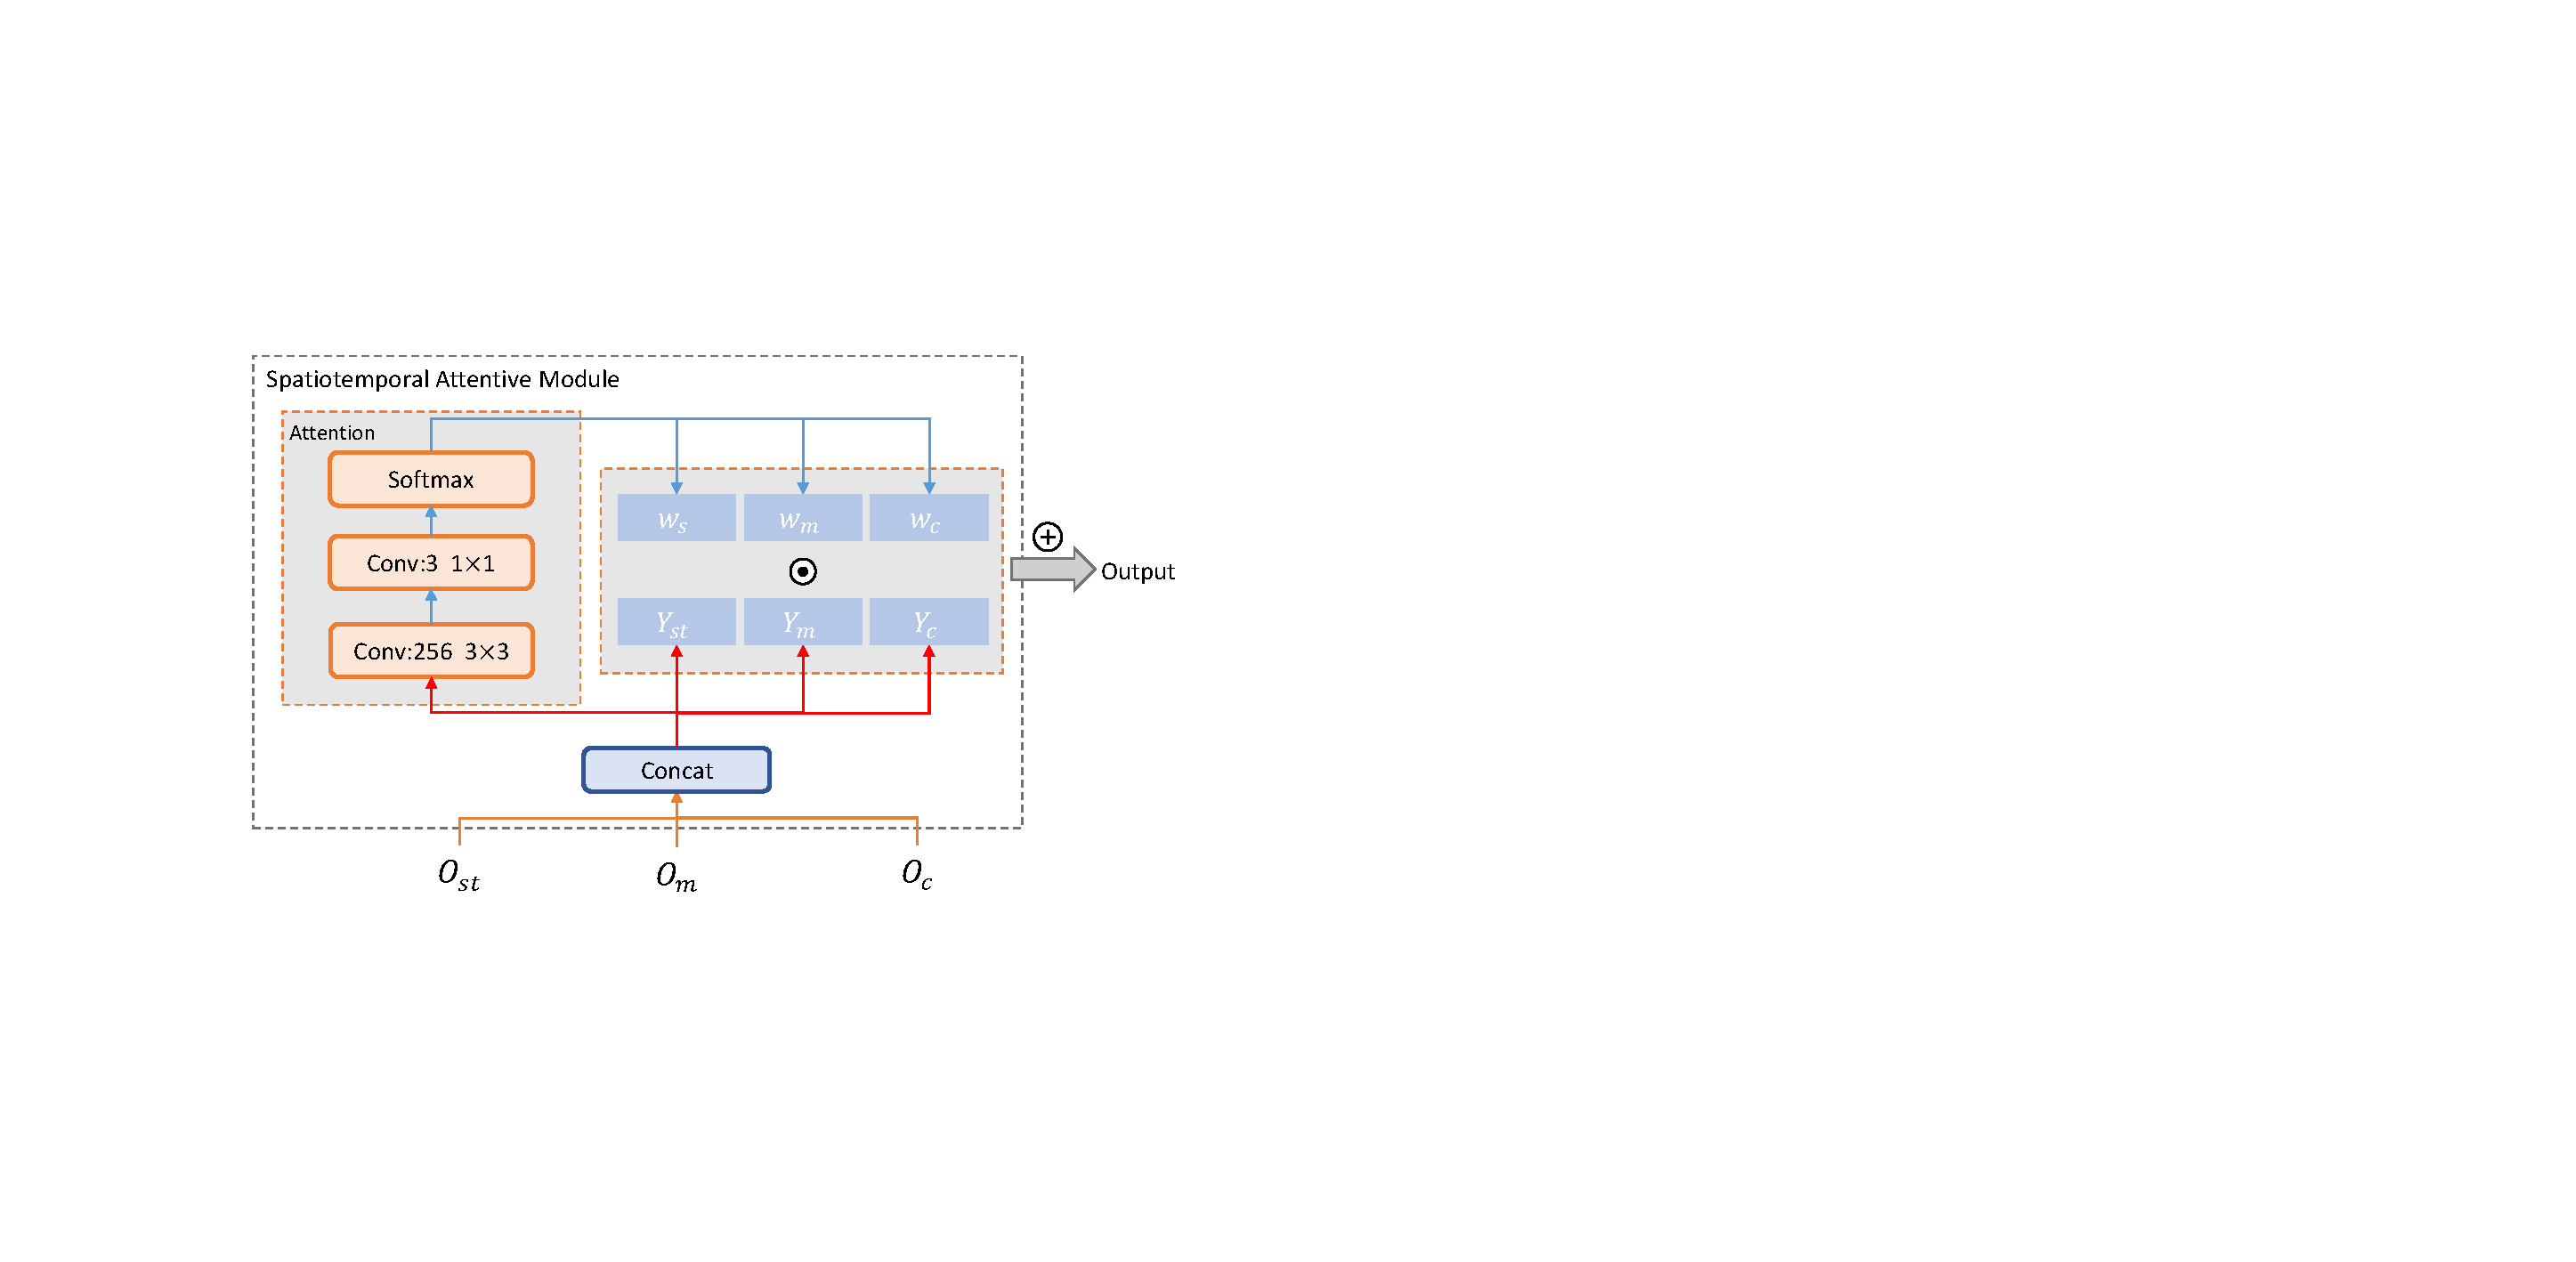
\includegraphics[width=8.5cm]{figures/attention}
\caption{时空注意力模块的具体结构}
\label{sta}
%\vspace{-5pt}
\end{figure}

在原有的多尺度ConvLSTM网络中,本文直接使用特征图求和来融合多类型的特征图。但是,直接求和的方式很难利用特征之间的上下文信息和相关性信息。因此,本文引入注意力机制来融合多类型特征,即把深度网络前端所产生的特征图$O_{st}, O_{m}, O_{c}$作为输入,然后使用图\ref{sta}的注意力模型进行相关性计算,这一个过程可以写作:
\begin{equation}
 \label{eq4_1}
 \begin{aligned}
   S  =  \sum_{a \in \{O_{st}, O_{m}, O_{c}\}} w_{a} \odot Y_{a}
   \end{aligned}
\end{equation}

其中$Y_a$表示的就是不同类型的特征图输入,而$w_a$则表示不同类型特征图对应的权重,其意义就是不同类型特征图的重要程度,即此注意力模块试图学到的参数。

通过图\ref{sta}中的具体结构,为了学习注意力权重参数,本文首先堆叠三种不同类型的特征图($O_{st}, O_{m}, O_{c}$),并把它输入进一个含有两个卷积层的小型神经网络,其网络配置是一个通道为256、卷积核为3$\times$3的卷积,另一个是通道为1、卷积核为1$\times$1的卷积。然后,特征权重由一个softmax激活函数归一化得到。最后,通过使用元素级相乘`$\odot$'和元素级相加`$\sum$'得到最终的显著预测结果$S$。

\subsection{粗标签的生成}
使用粗标签的动机是因为在SCNN中所使用的并行弱监督迭代策略存在一些瑕疵,即在训练过程中生成弱标签无法应对复杂场景,生成的弱标签存在不少的背景噪声,这些噪声会直接影响深度网络的学习。最直接的解决方法仍是手工标定准确的像素级标签,但是这一个方法工作量巨大,而且标定视频显著目标还需要眼动仪这类硬件支持,所以本文没有直接标定精细的像素级标签。然而,通过标定尝试,本文发现直接标定工作量大,但是如果已经有了弱标签,我们在其上进行修正,即把背景噪声擦除,这样的标签也能对网络训练有辅助作用,并且这样的方法不需要过多的工作量。这些先由显著性方法生成,再手工擦除的像素级标签,本文称之为粗标签。

\begin{figure}
 \centering
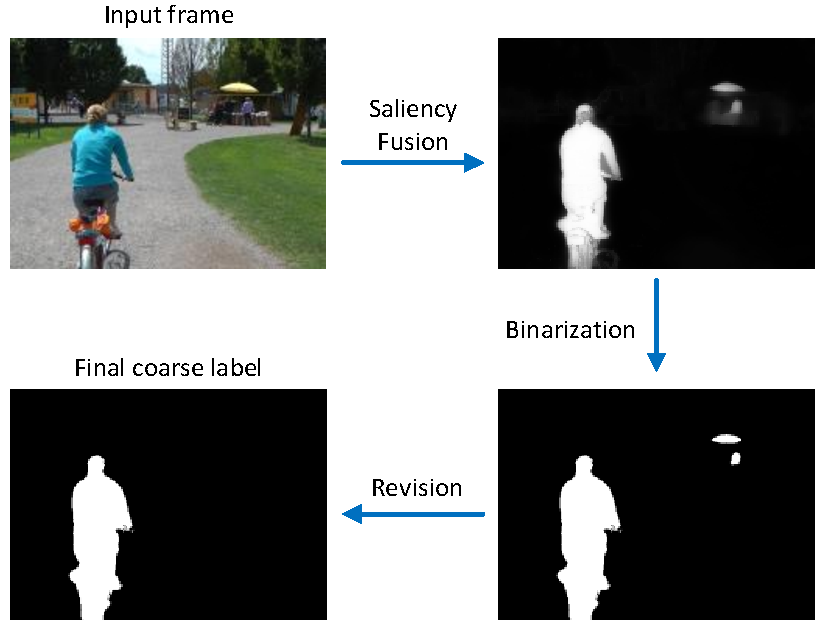
\includegraphics[width=9.5cm]{figures/labeling2}
\caption{粗标签的产生流程}
\label{labeling2}
%\vspace{-5pt}
\end{figure}

粗标签的生成流程如图\ref{labeling2}所示,方法直接简单,总共四个步骤:首先,把待标记的视频帧用图像显著性检测的方法检测出主体的显著目标。这里本文选择了三个准确率较高的基于深度学习的图像显著检测方法(DCL \cite{li2016deep}, RFCN \cite{wang2016saliency}, DSMT \cite{li2016deepsaliency})。第二步,使用加权求和的方式,把三个方法检测到的显著图融合成一张。权值的求解与SCNN的并行迭代弱监督训练中的一样,仍是使用最小二乘方法求解。求解时使用的真值是FBMS自带手工标定的像素级标签。第三步是图像二值化。设置一个阈值,把融合的显著图转化为二值图像。这里选定的预测为128,即显著图中的像素值超过128的,设置为前景正样本,给定标签为1;像素值不足128的,设置为背景负样本,给定标签为0。第四步,擦除背景区域。图像显著性检测方法检测的结构不论如何准率,但是运用于视频序列上仍有不足,例如图\ref{labeling2}中的右上角亮斑。因此,本文利用手工擦除的方法,移除这些较为明显的背景噪声区域,从而生成相对准率的粗标签。通过粗标签标定,本文快速地收集到了足够的训练数据(共3326帧)来完成网络训练。


\section{实验结果和分析}
在此结中,本文首先简单介绍一下使用到的数据集合评价方法。其次,详细介绍本文在实现注意力融合时空深度网络(STAN)时需要注意到的一些细节。接着,本文给出与其他显著性方法的详细对比。在这之后,STAN网络中的各个模块会用实验的方式一一进行验证它们的有效性。最后,本文也会对STAN进行算法效率上的分析。

\subsection{实验数据集和评价方法}
在本章中使用到的数据集与前一章相近,共使用到SegTrackV2、FBMS、DAVIS三个数据集进行实验验证。与前一章数据集的差别在于,在网络训练时,本章的训练数据一共含有51个视频序列,共6098帧,分别是一半的DAVIS数据、含有粗标签的FBMS训练集和所有的SegTrackV2数据。而在测试中,另一半的DAVIS数据和FBMS的测试集则被用来验证STAN的有效性。

在评价方法方面,本章与上一章相同,采用准确-召回曲线(precision-recall curve)和平均绝对误差(mean absolute error)在上述数据集上验证本章方法,具体的结果将在下一个小节中展示。

\subsection{具体实现}
为了训练得到一个有效的神经网络和获得高鲁棒性的时空深度特征,本文在实现STAN时,需要注意下列几点细节:
\begin{itemize}
  \item 由于基础网络仍是VGG型的全卷积网络,本文使用ImageNet的模型参数来初始化。同时,由于时间子网的输入是一个四维张量(三维视频帧和一维运动先验),其第一个卷积层需要使用高斯分布重新初始化。
  \item 在STAN网络中,为了在两个子网流中提取多尺度特征,本文设计了一些网络分支。每个子网中有两个分支,一个嵌入在第四个pooling层后,另一个嵌入在网络最末端的卷积层后。
  \item 在训练阶段,由于GPU显存的限制,输入图像的尺度被设定为512$\times$512,而且网络的batch size被设定为4。
  \item 在网络测试阶段,与SCNN的方法一样,同样引入稠密条件随机场(dense-CRF)\cite{chen2014semantic}作为后处理方法,进而提高显著图的空间一致性和质量。
  \item 本文采用的Adam(Adaptive Moment Estimation)算法作为整个网络的优化算法。整个STAN网络的初试学习率(learning rate)被设定为$10^{-3}$
\end{itemize}

\subsection{方法对比}
在本节中,为了证明本文提出STAN的优势,本文分别在FBMS和DAVIS两个数据集上对比了16个近期方法,其中6个视频显著性检测方法,10个图像显著性检测方法,各方法的细节如下:

\begin{itemize}
  \item CS算法\cite{fu2013cluster},即Co-Saliency协显著性检测方法,通过聚类的方式,找寻连续视频帧之间的相关性,进而完成视频显著性检测。
  \item ST算法\cite{zhou2014time},为了抑制视频序列中的动态模糊问题,该算法利用从高帧率到底帧率的动态匹配来完成视频显著性检测。
  \item SS算法\cite{rahtu2010segmenting},结合的统计学框架和各类局部特征(如光照、颜色、运动信息)来进行显著性估计,并使用CRF信息显著图修正。
  \item SA算法\cite{wang2015saliency},基于无监督测地线距离(geodesic distance)的显著性检测方法,利用空间与时间运动边界的约束,用测地线距离来区分前景与背景区域。
  \item CG算法\cite{wang2015consistent},基于梯度光流域和能量优化函数,结合帧内边界信息和帧间运动信息来推测目标显著性。
  \item DLVS算法\cite{8047320},该方法是较早使用深度模型的方法,利用两个子网的衔接,运动特征是把连续两帧叠加输入网络学习得到。
  \item RFCN算法\cite{wang2016saliency},图像显著性检测方法,利用循环结构迭代生成显著图。
  \item DCL算法\cite{li2016deep},图像显著性检测方法,基于DeepLab模型\cite{chen14semantic},并在其基础上加入多尺度深度特征,从而使得网络在利用高层语义特征做主要显著性估计的同时,可以利用低层特征弥补目标边界的不足。
  \item MDF算法\cite{li2016visual},图像显著性检测方法,采用多层次分割图像获得超像素,并利用超像素的深度特征训练一个二分类器来判断超像素显著与否。
  \item DSMT算法\cite{li2016deepsaliency},图像显著性检测方法,网络是基于VGGNet,但是在优化时不仅使用常用的二元交叉熵目标函数,还引入L2目标函数进多任务优化。
  \item DSS算法\cite{DSSalCVPR2017},图像显著性检测方法,网络采用特征图短连接的方式结合,属于稠密连接的方法,可以获得鲁棒性很高的深度特征。
  \item DHSN算法\cite{liu2016dhsnet},图像显著性检测方法,网络不仅使用了多尺度特征图提取,而且还引入了recurrent循环结构进行特征优化。
  \item Amulet算法\cite{Zhang_2017_ICCV_Amulet},图像显著性检测方法,聚合多层级特征网络,即在深度网络中把多个卷积块的特征都提取出来做融合,再利用融合特征做显著性估计。
  \item WSS算法\cite{Wang2017Learning},图像显著性检测方法,考虑到训练数据不足问题,把图像有的分类标签也引入显著性网络进行学习。
  \item UCF算法\cite{Zhang_2017_ICCV_UCF},图像显著性检测方法,该深度网络提出一张新型的reformulated dropout来解决特征图中的内部单元不确定结合。
\end{itemize}

此外还有上一章节提出的级联神经网络SCNN,本章提出的多尺度时空ConvLSTM网络MSST和时空注意力融合网STAN。

\begin{figure*}
\centering
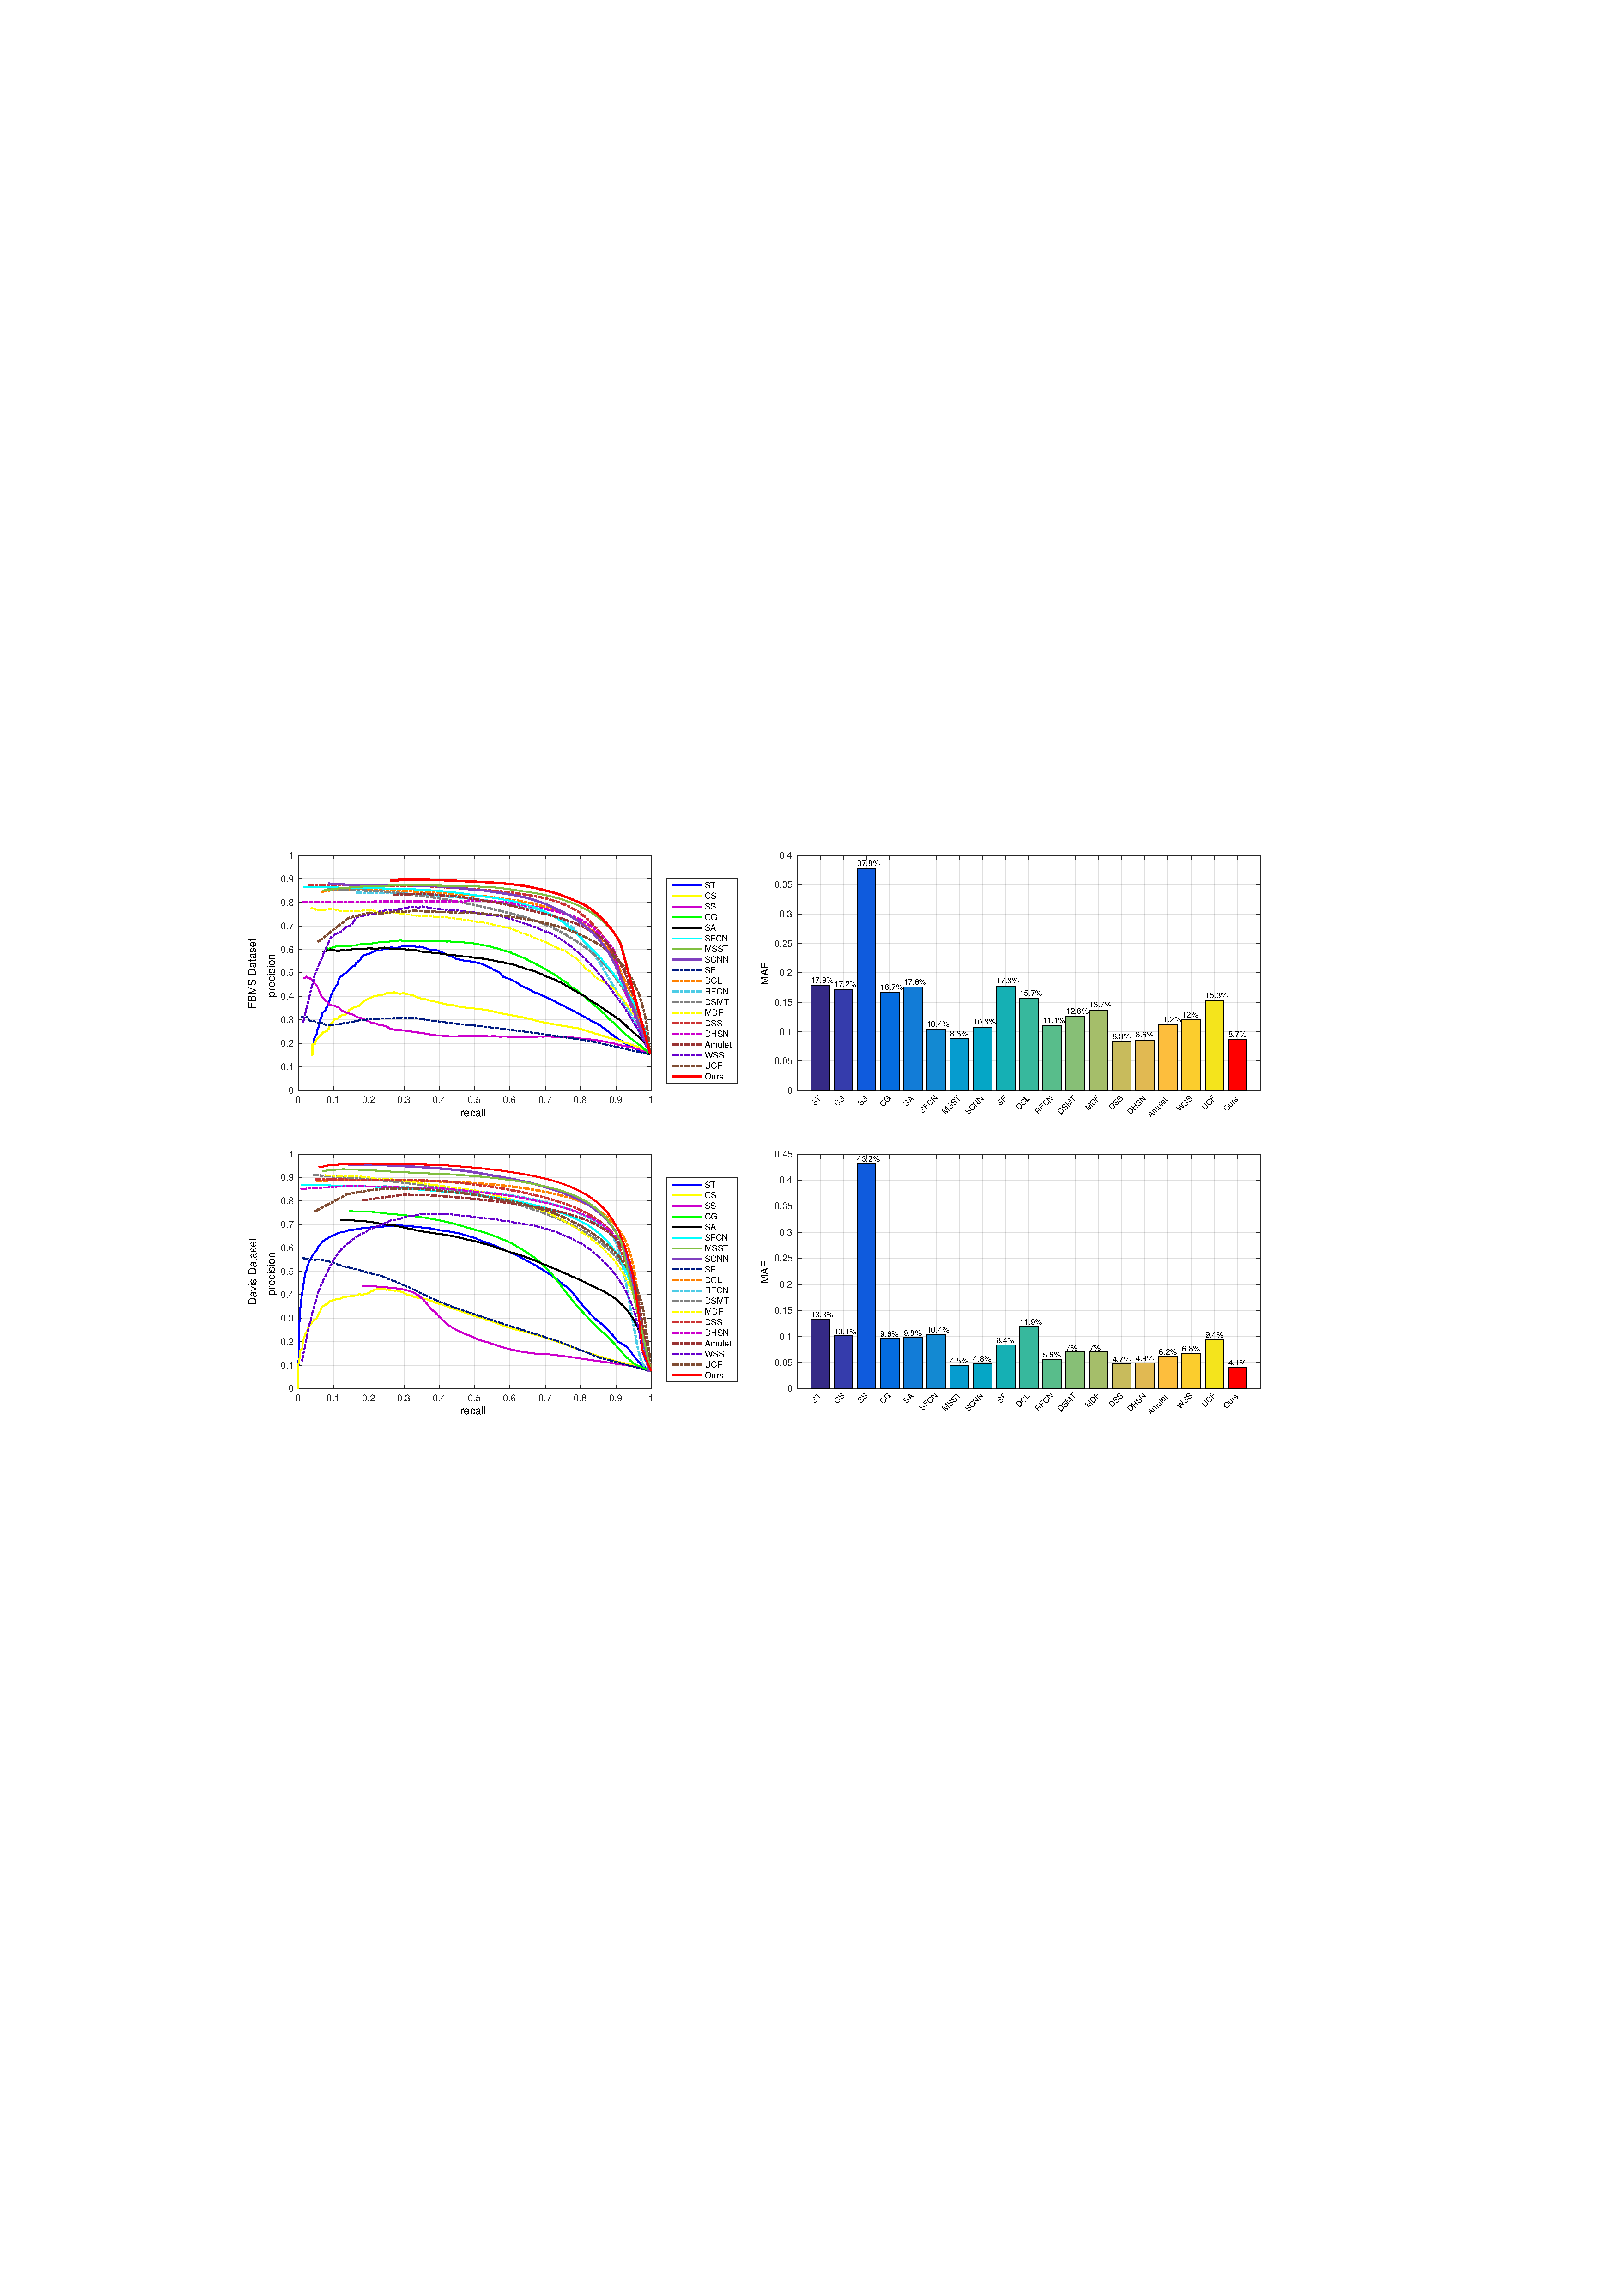
\includegraphics[width=1\textwidth]{figures/methos_compare_new3}
\caption{本章方法与其他方法的定量比较;比较方法包括8个视频显著性检测方法(实线)和10个图像显著性检测方法(虚线),左栏是PR曲线,而右栏是MAE柱状图}
\label{figure4}
\end{figure*}

所有方法的PR曲线和MAE柱状图的结果如图\ref{figure4}所示。从图中我们可以看到,本章提出的MSST和STAN都取得了有竞争力的结果。MSST在FBMS和DAVIS分别取得8.8\%和4.5\%得结果;PR曲线的表现也很好,从左图的右上角可以看出,MSST已经超过了大多数方法。STAN由于引入的更为多样的运动特征精炼模块和注意力特征融合模块,MAE和PR曲线更进一步提高,MAE在FBMS和DAVIS中达到了8.7\%和4.1\%,在PR曲线上则提高得更明显。

\begin{figure*}
\centering
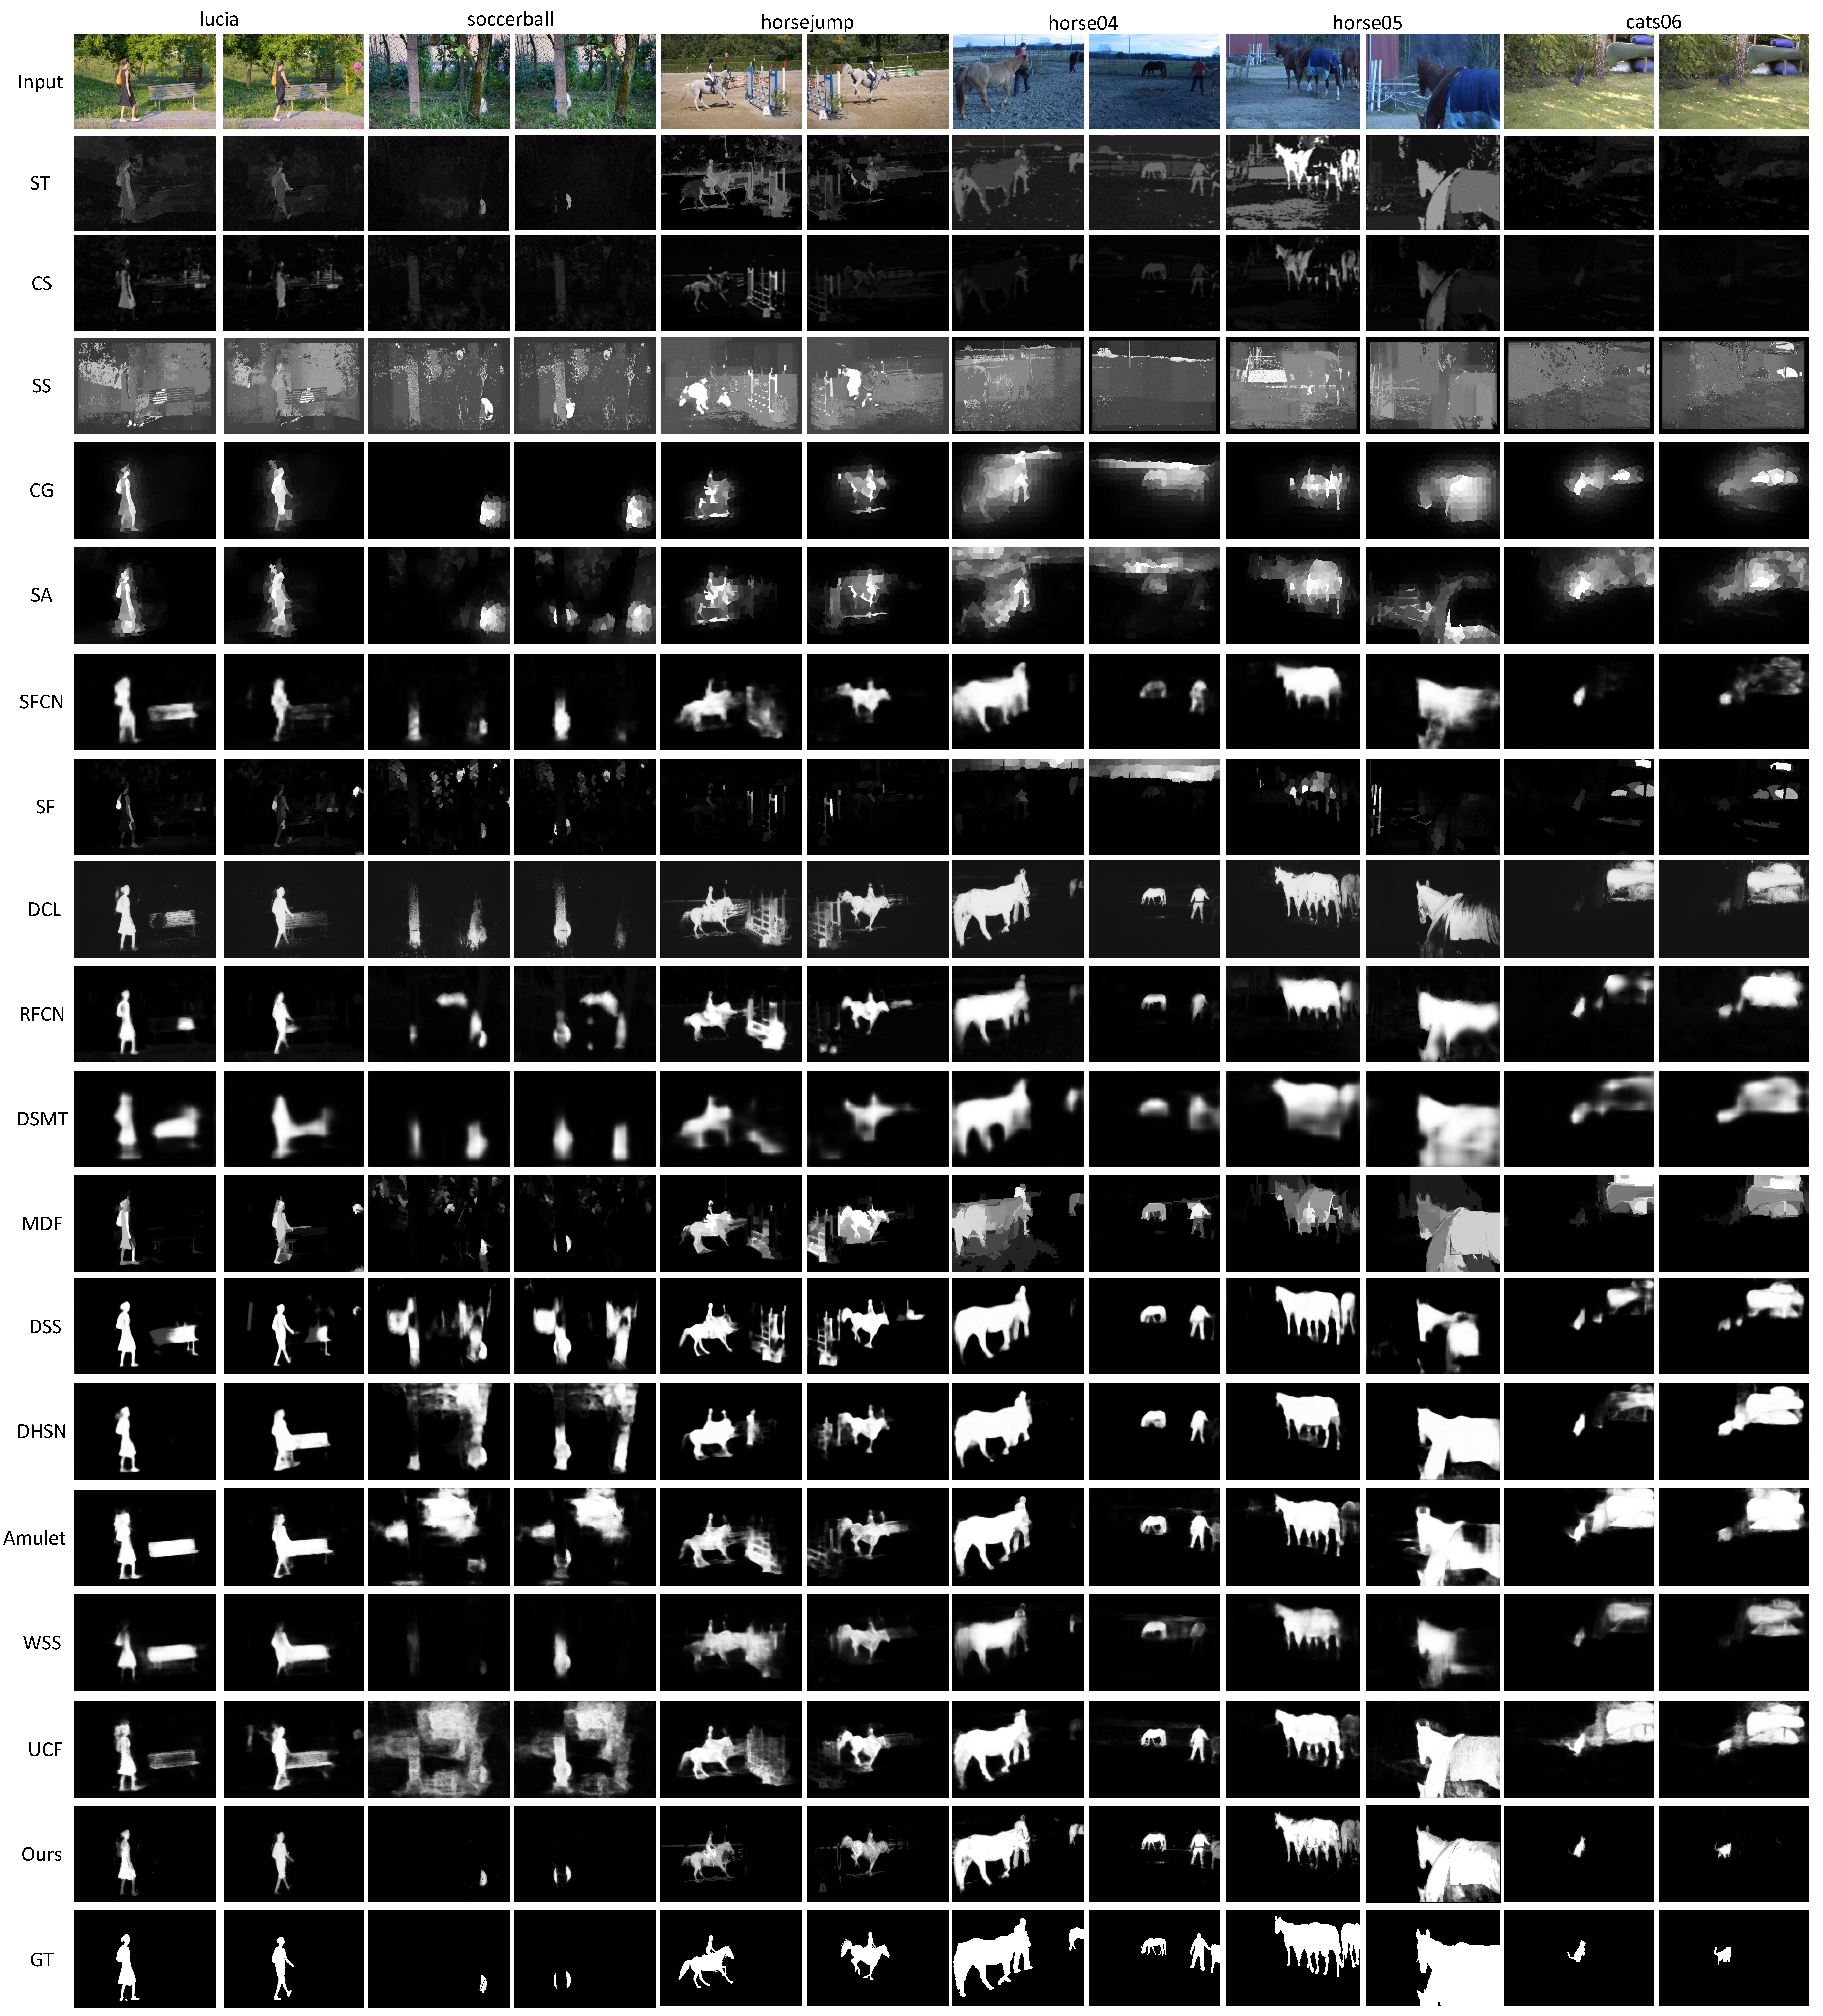
\includegraphics[width=1\textwidth]{figures/show}
\caption{本章方法与其他方法的定性比较,其中左边三栏的显著图来自DAVIS数据集,右边三栏来自FBMS数据集}
\label{figure5}
\end{figure*}

图\ref{figure5}展示的是所有方法在FBMS和DAVIS生成显著图。前三个序列(lucia、soccerball、housejump)来自DAVIS数据集。后三个序列(horse04、horse05、cats06)是来自FBMS数据集。通过这些显著图结果的观察,可以总结出本文提出方法的三个亮点:

首先,可以处理多显著目标的视频序列。horse04和horse05序列即包含多显著目标。一些方法只能够检测出一部分显著目标,而本文提出的方法充分地融合静态与运动的时空特征,可以高亮在这样多目标的序列中高亮所有的显著目标。

其次,可以处理小目标和被遮挡目标。在一些视频序列中,如soccerball,显著目标很小,甚至被背景区域遮挡,这样就导致大部分显著性检测方法都会失败。而本文提出的方法由于合适的深度网络结构和足够训练数据,可以很好地处理这一特殊情况。

最后,本文提取到了良好的运动特征和利用合适的方法进行了特征融合。在提出运动特征是,本文利用到了光流、ConvLSTM、三维卷积等方法,获得了相对较为丰富的运动特征。同时,本文利用基于注意力机制的特征融合模块进行多类型特征融合,得到的特征可以准率地检测出运动显著目标和尽可能地消除对比度高的背景噪声区域(如,lucia序列中的长凳)。
\subsection{各个子模块的有效性验证}
在前文中,本文提出的STAN包括五个模块,分别为:空间子网流、时间子网流、ConvLSTM模块、三维卷积模块和时空注意力特征融合模块。为了验证各个模块的有效定,在这一小节中,本文分别设计了相应的实验来验证它们的有效性。首先,本文针对STAN中的网络配置做了验证:

\begin{itemize}
  \item \textbf{OS}:只使用空间子网流(即单个FCN模型)来估计视频帧的显著性。由于网络的局限,在训练网络时只能把视频帧当做图像来进行网络训练,因此该配置没有引入运动特征。
  \item \textbf{ST}:双子网流都被利用来提取多尺度时空特征。并且,在网络的末端,特征图融合使用的是直接求和的方式。
  \item \textbf{STL}:这一个网络配置即为本章前面提出的MSST框架,把双流子网生成的多尺度特征图送入ConvLSTM进行运动特征精炼,然后采用直接求和的方式进行特征融合,从而生成最终的显著图。
  \item \textbf{STLC}:在STL的基础之上,加入三维卷积运算,与ConvLSTM一起组成运动特征精炼模块,生成不同类型的深度特征图。这些不同类型的特征会在网络末端使用直接求和进行融合。
\end{itemize}

\begin{figure}
\centering
\subfigure[逐渐引入本章提出网络模块的实验比较]{
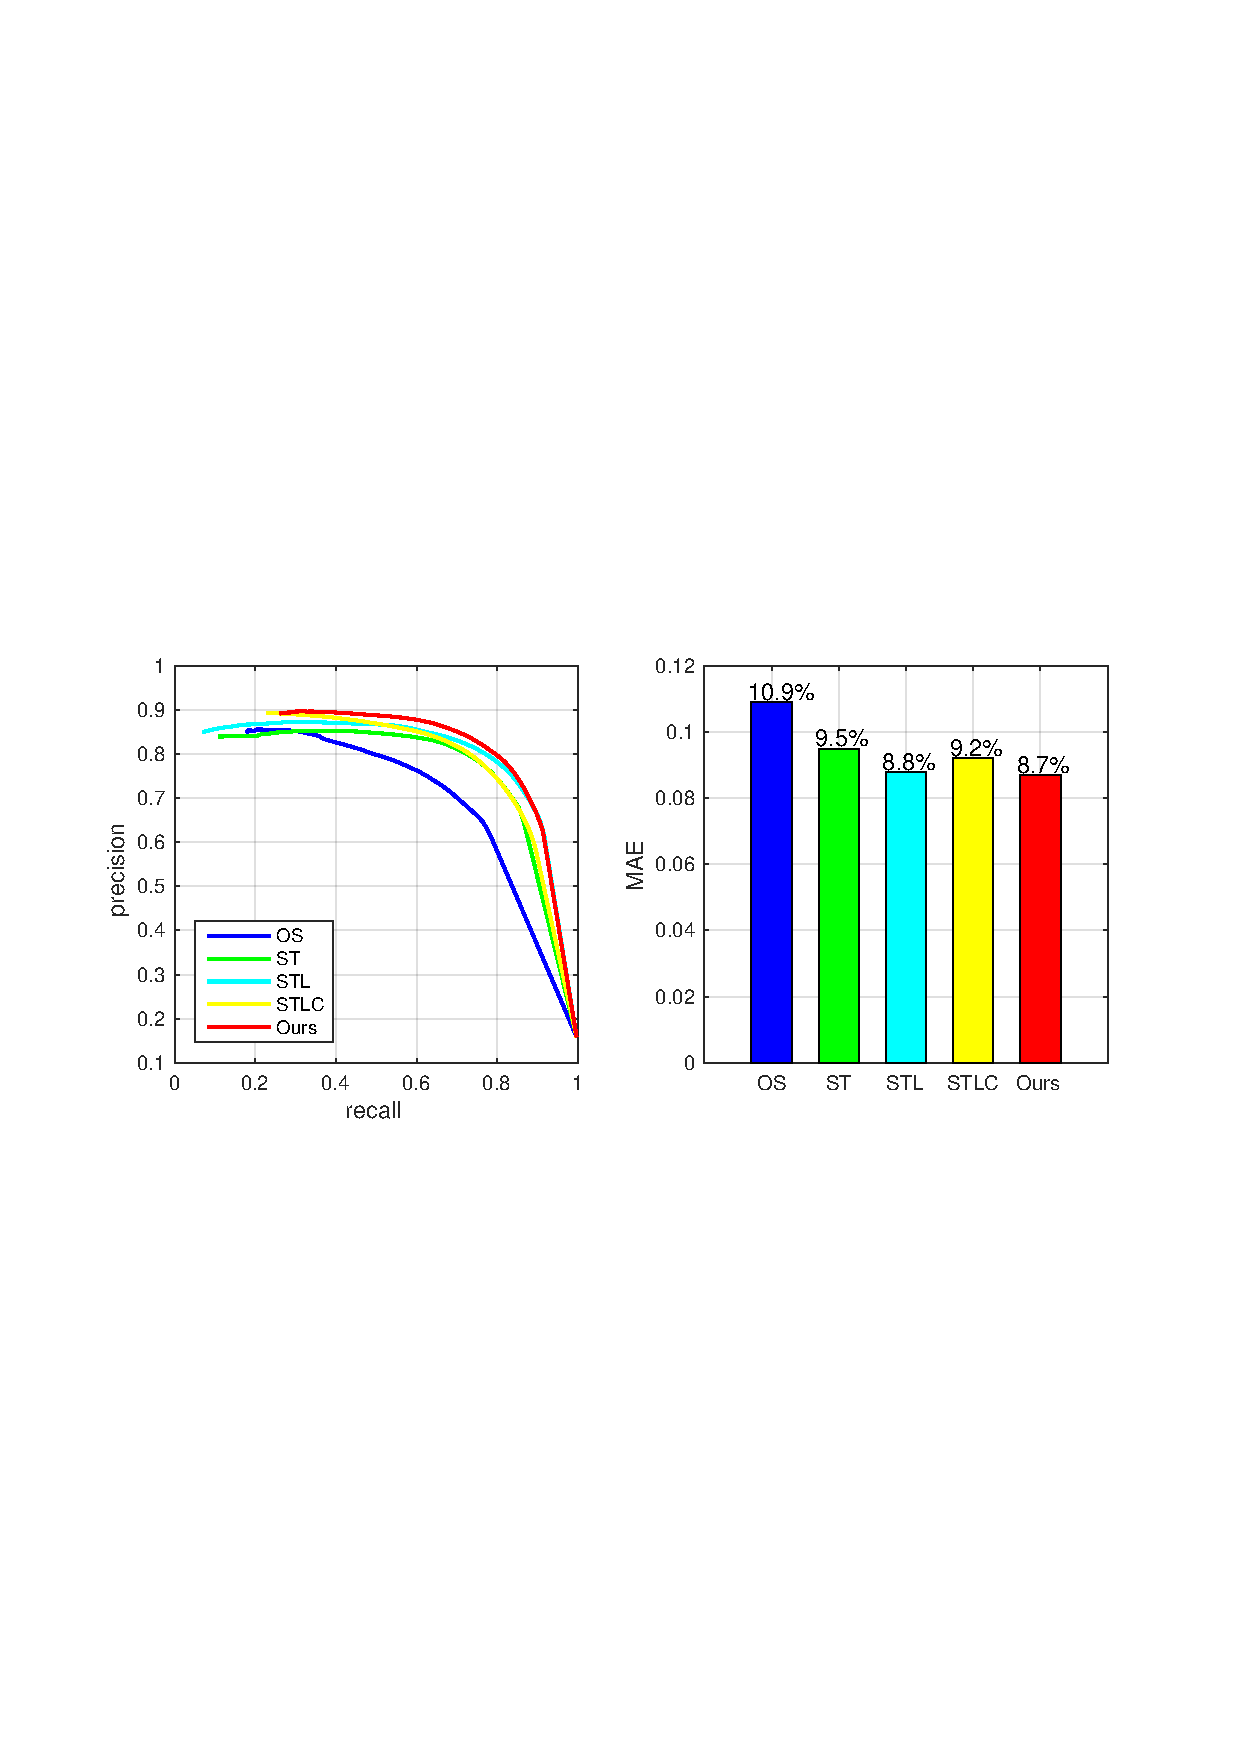
\includegraphics[width=10.7cm]{figures/self_compare_config}
}
\subfigure[使用和不使用粗标签训练网络的实验比较]{
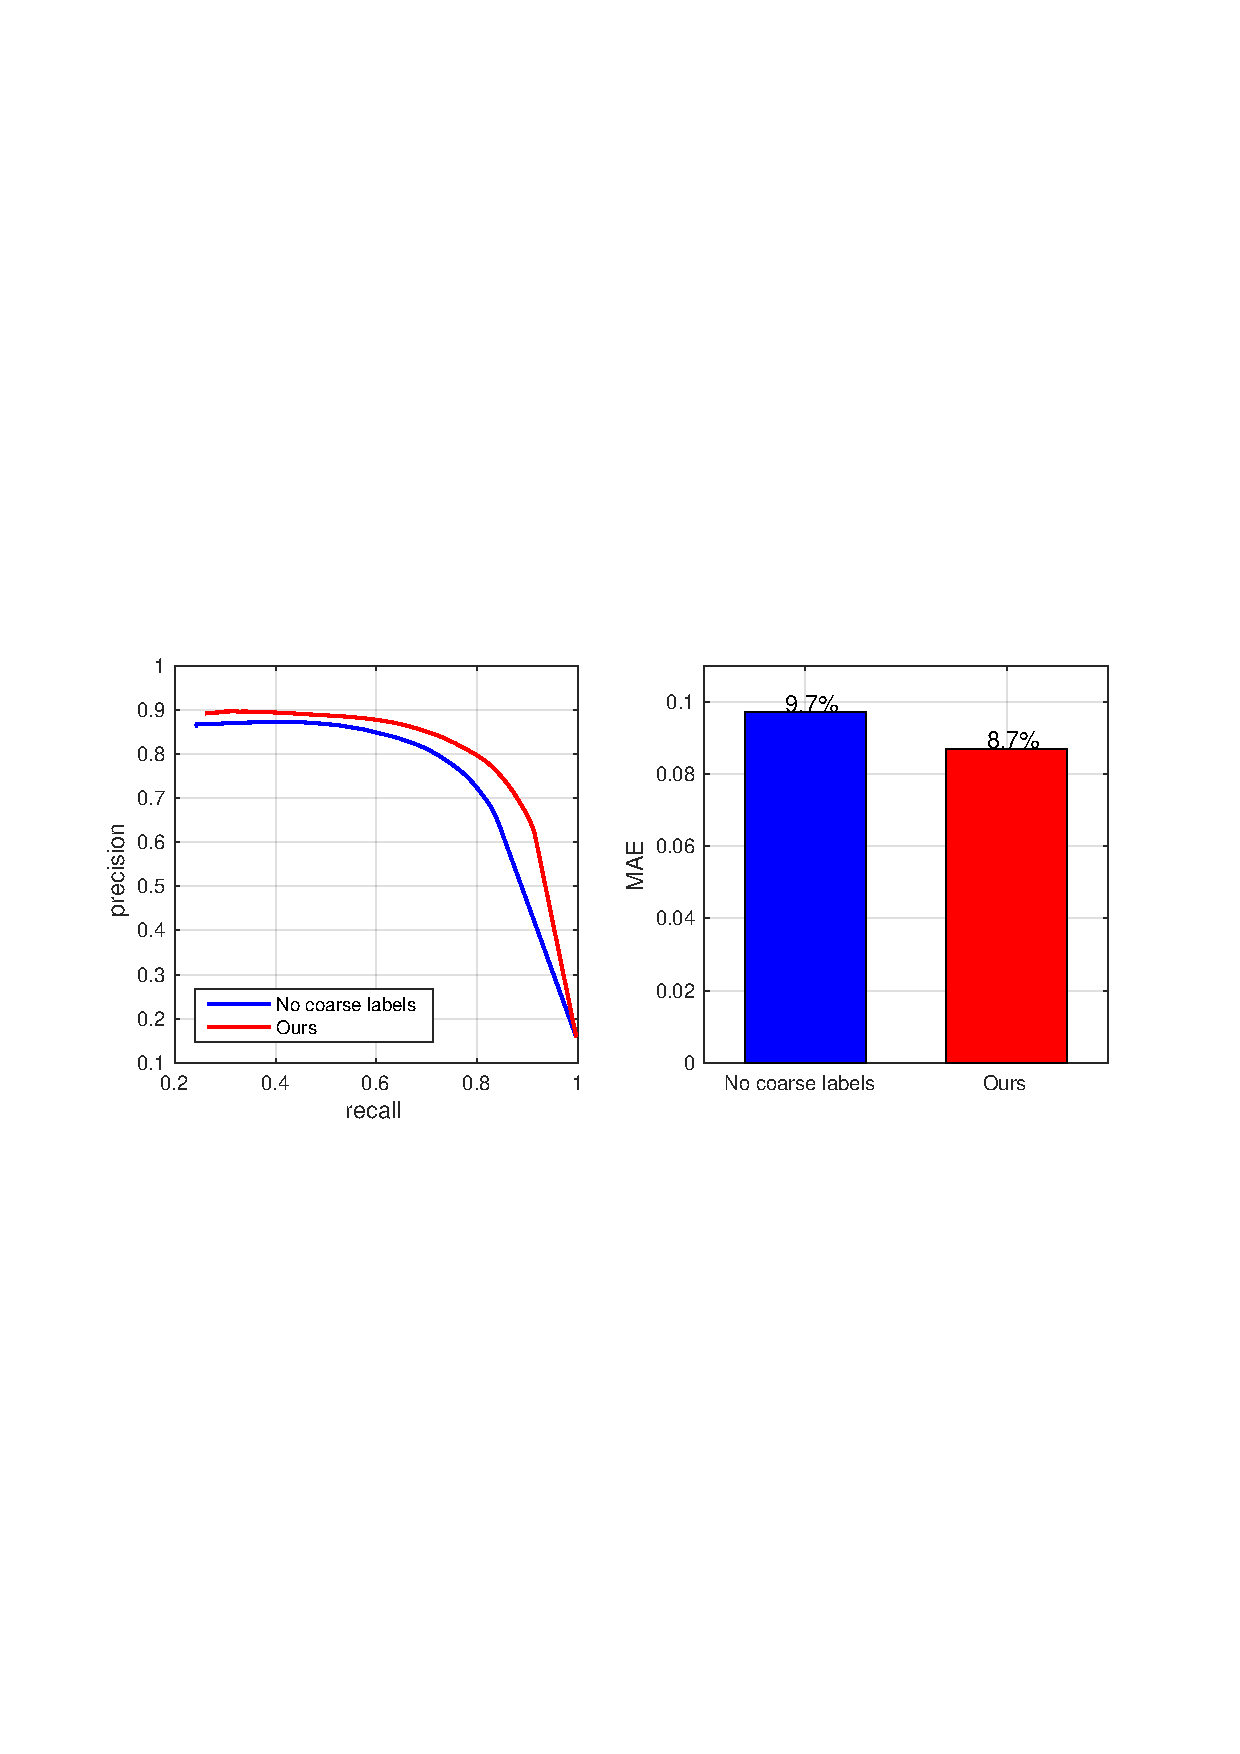
\includegraphics[width=10.7cm]{figures/self_compare_coarse}
}
\subfigure[直接使用光流作时间子网输入和使用视频帧与运动先验堆叠作输入的实验比较]{
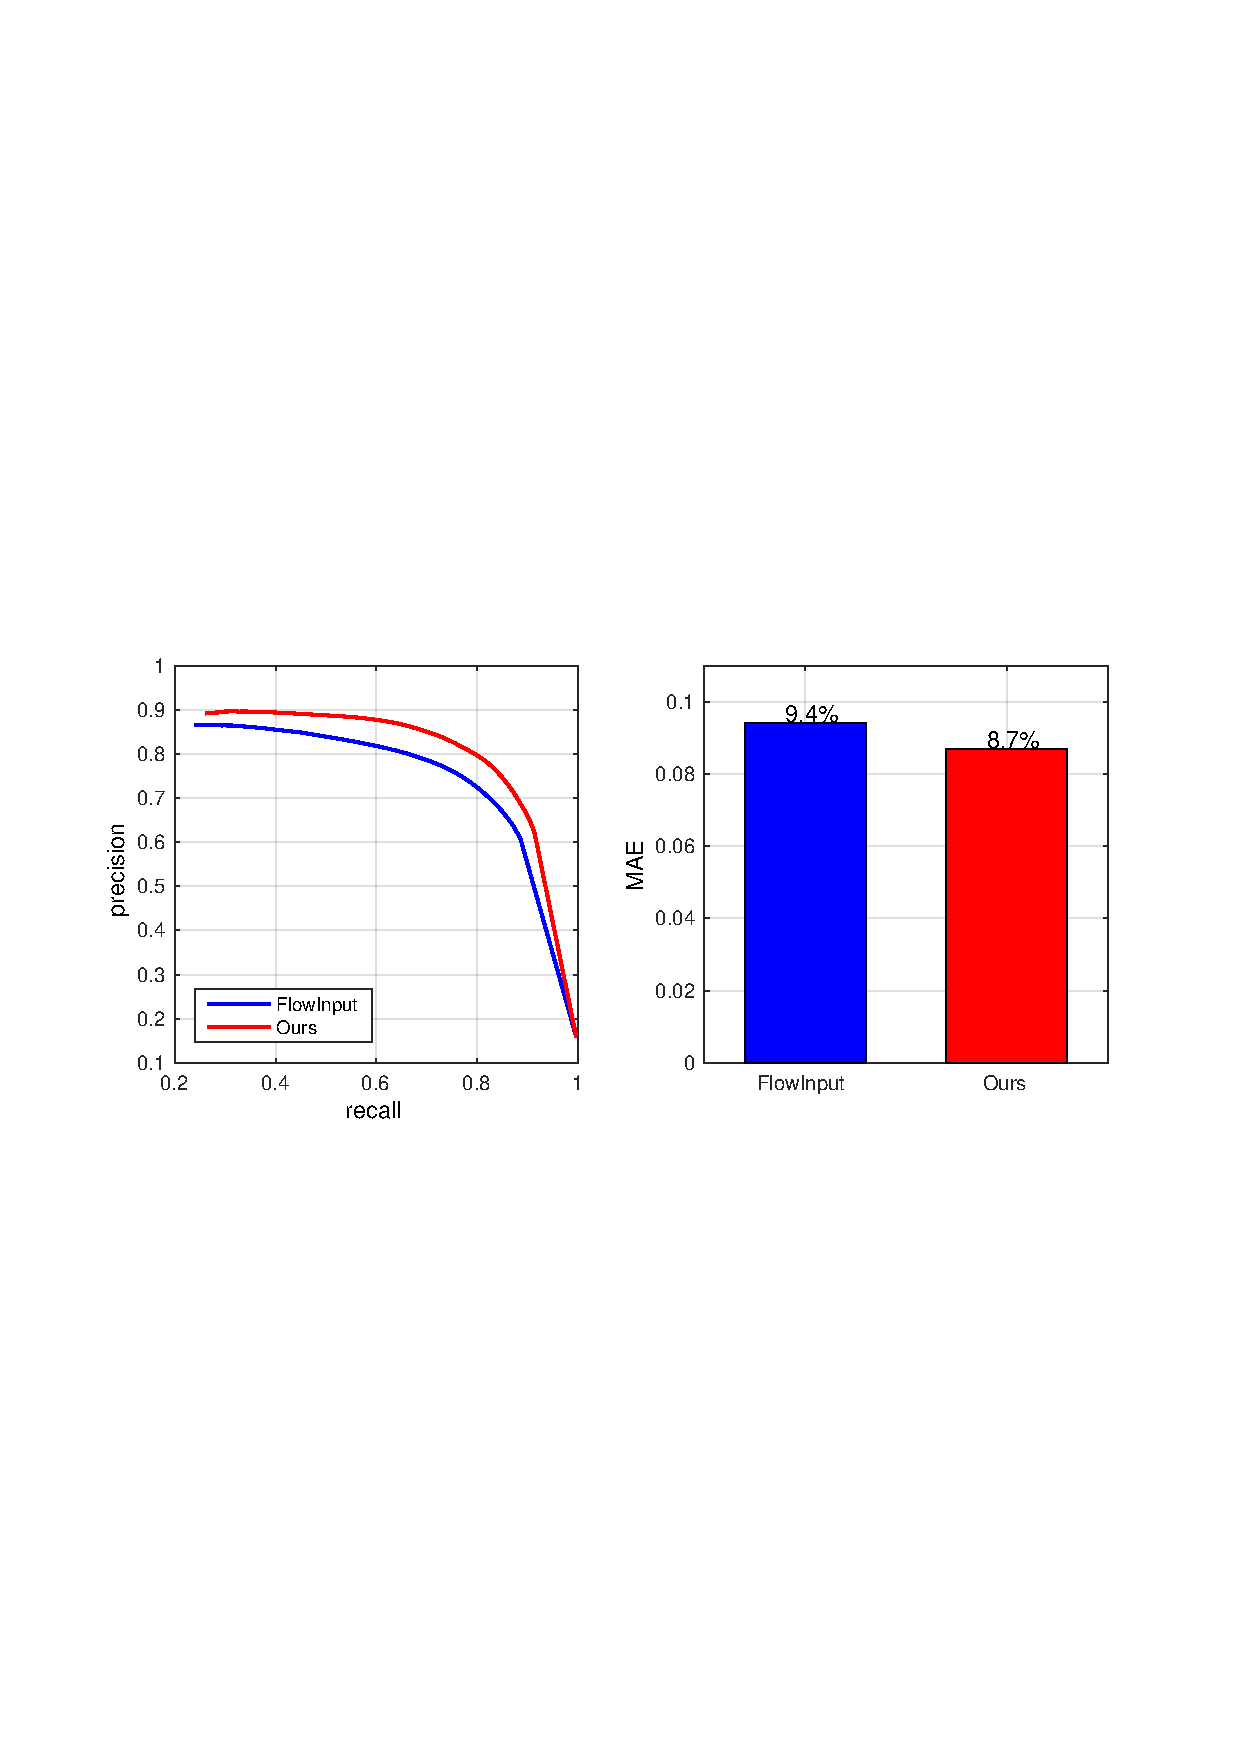
\includegraphics[width=10.7cm]{figures/self_compare_flow}
}
\caption{不同网络配置的定量分析}
\label{diff_config2}
\end{figure}

模块验证的定量实验结果如图\ref{diff_config2}(a)所示,本文一步步地把网络结构合理化并逐步验证其有效性。首先,本文只使用空间子网流做显著性预测。由于缺少运动特征,其结果存在严重的缺陷。之后,本文结合使用的空间子网和时间子网,这一个改进的结果使得实验的表现都有很大的提高。接着,本文又加入ConvLSTM模块精炼运动特征,在一定程度上,PR曲线和MAE又有一定地提升。然而,随着三维卷积运算的引入,PR曲线虽然在准确率端有微小的提高,但是在召回率端和MAE上的表现反而没有上一个配置好。分析其原因,本文认为是直接使用特征求和的方式很难融合不同类型的特征图。并且,不同类型特征之间的上下文信息和相关性信息没有充分利用。因此,本文引入 的注意力时空特征融合模块来解决这一个问题。而且从图中的曲线和柱状图也可以看出,本文提出了一个方法是有效的。在图\ref{config}中,本文也展示了不同网络结构生成的显著图结果,从直观上验证本文提出的方法。

\begin{figure*}
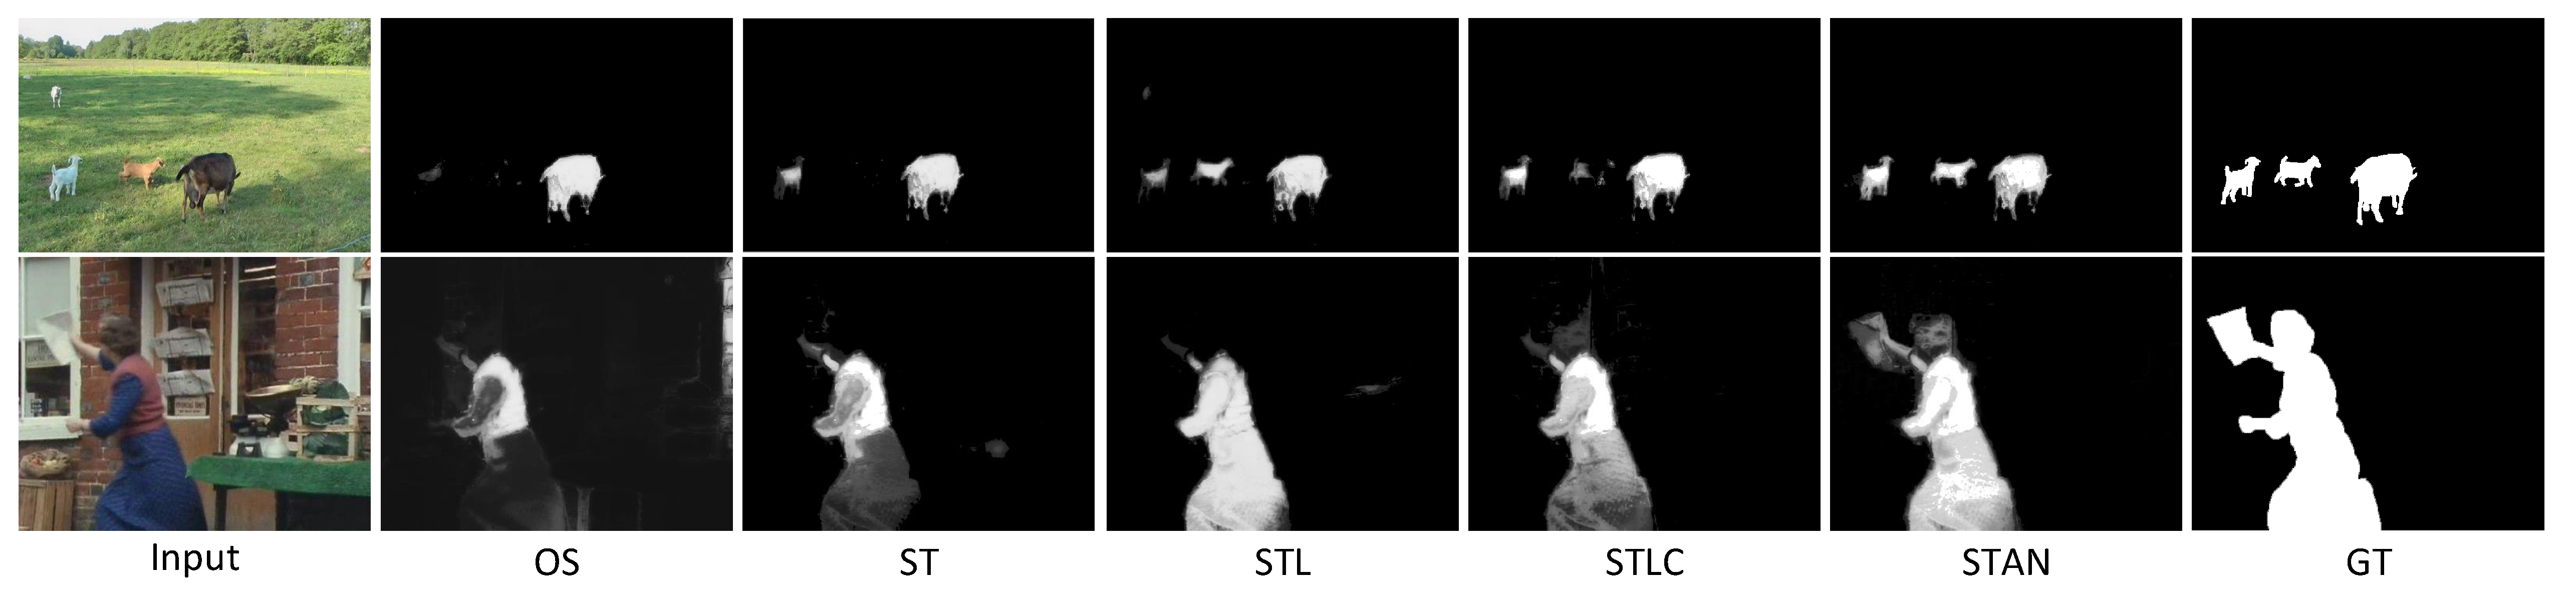
\includegraphics[width=1\textwidth]{figures/show_config}
\caption{不同网络配置下产生的显著图。从左到右依次是只使用空间子网的结构(OS)、结合空间与时间子网的结构(ST)、加入ConvLSTM模块后的结构(STL)、加入ConvLSTM与三维卷积后的结果(STLC)、本章提出的完整结构(STAN)}
\label{config}
%\vspace{-5pt}
\end{figure*}

为了证明粗标签对网络训练的有效性,本文针对使用和不使用粗标签设计一个对比实验,其实验结果如图\ref{diff_config2}(b)所示。可以看到,使用粗标签网络的PR曲线与MAE柱状图都比不使用粗标签的要好很多。而且,引入了粗标签后,STAN网络的训练数据可以从2772个样本直接上升到6098个样本,增加了一倍多。此外,一些复杂场景的数据也加入到训练集中,这些数据可以让神经网络学到更为丰富的特征,从而提高显著估计的准确率。

在STAN网络中,空间子网的输入是一个四通道的图像,即把视频帧与基于光流分割的运动先验图堆叠在一起。为了验证这种输入的优势,本文设计了一个实验,对比的是即采用视频帧与运动先验的堆叠和原始的光流特征图。实验的PR曲线和MAE柱状图如图\ref{diff_config2}(c)所示,可以看到,四通道先验堆叠的输入明显比用光流输入的结果好。

\subsection{时间效率分析}

本文的所有实验都在一个GPU工作站上进行,其配置是一个Intel(R)i7-5820 CPU (3.3 GHz),一个Nvidia Geforce TITAN X GPU (12GB显存)和64G内存。表\ref{table4}和表\ref{table5}分别展示了不同方法在DAVIS数据上的平均运行时间和本文提出方法在每一个模块消耗的时间。可以看到,由于需要提取光流SS、SA、CG的运行时间都很长。本章提出的STAN为了提取运动先验也使用到了光流图。为了加快光流图的提取,本文没有使用传统的光流提取法\cite{Sun2014A},而是引入了FlowNet2.0\cite{8099662},即保证了光流图的质量,也加快了提取速度。从数值上看,FlowNet2.0可把光流图的提取速度提高到0.739秒每帧。因此,STAN最终的计算速度是2.144秒每帧。

\begin{table}
%\scriptsize
\centering
\caption{DAVIS数据上各方法运行的平均时间(秒每帧)}
\renewcommand{\arraystretch}{1.0}
%\begin{tabular}{|l|p{0.8cm}|p{0.95cm}|p{1.0cm}|p{1.05cm}|p{0.99cm}|}
\begin{tabular}{|c|c|c|c|c|c|c|}
\hline
\hline
Method &STAN  &ST  &CS  &SS    &CG  &SA\\
\hline
Time(s) &2.144  &28.193 &1.175   &37.176  &38.075 &38.751\\
\hline
\hline
Method    &DLVS  &SF   &DCL    &RFCN   &DSMT   &MDF  \\
\hline
Time(s)    &0.473 &0.842 &0.670   &4.580  &0.14    &11.33    \\
\hline
\hline
Method      &DSS  &DHSN   &Amulet   &UCF  &WSS  & \\
\hline
Time(s)    &0.453  &0.465   &5.299   &0.151 &0.024 & \\
\hline
\end{tabular}
\label{table4}
\end{table}

\begin{table}
%\scriptsize
\centering
\caption{本章提出方法在各个模块上消耗的平均时间(秒每帧)}
\renewcommand{\arraystretch}{1.0}
\begin{tabular}{ |l|l|r|r| }
%\hline
%\multicolumn{3}{ |c| }{Time sheet} \\
%\hline
\hline
\hline
Model & Component & Time (s) & Ratio (\%)\\ \hline
\multirow{5}{*}{STAN} & Optical flow computation & 0.739 & 34.5\\
 & Motion prior generation & 0.823 & 38.3\\
 & Neural network processing & 0.102 & 4.8\\
 & Saliency refinement & 0.480 & 22.4\\\cline{2-4}
 & Total & 2.144 & 100\\ \hline

\end{tabular}
\label{table5}
\end{table}
\section{小结}
在本章中,本文提出了两种深度模分别是多尺度ConvLSTM模型和注意力时空特征融合模型,后者是前者的扩展,都是采用了双子网流模型,分别用于提取多尺度的空间与时间特征。同时,本章为了获得更为鲁棒的运动特征,提出了一个运动特征精炼模块,采用ConvLSTM和三维卷积来挖掘视频序列中的运动特征。此外,本章还引入了一个基于注意力机制的多类型特征融合模型,把时空特征进行了有机融合,进而生成准确率高的显著图。考虑到网络训练数据不足和弱标签的背景噪声问题,本章通过融合图像显著图和手工擦除背景噪声的方法标记了足够量的视频粗标签,从而使得网络训练可以有足够的数据支持。最后,本文STAN的实验结果在FBMS和DAVIS两个数据集中都取得了具有竞争力的结果。